\documentclass[a4paper]{article}

%%%%%%%% BIBLIOGRAPHIE %%%%%%%%
%\usepackage[backend=biber]{biblatex} %Imports biblatex package  //version biber et pas biblatex, ne marche pas direct sur texmaker.
%\addbibresource{biblio.bib} %Import the bibliography file

%%%%%%% PACKAGE %%%%%%%%%%%

\usepackage[utf8]{inputenc}
\usepackage{xcolor}
\usepackage{amsmath}
\usepackage{amssymb}
\usepackage{amsfonts}
\usepackage{verbatim}
\usepackage{amsthm}
\usepackage{geometry}
\geometry{hmargin=2cm,vmargin=1.5cm}
\usepackage{hyperref} %Références cliquables

%%%%% Pour les dessins %%%%%

\usepackage{tikz}
\usetikzlibrary{shapes,positioning}
\usetikzlibrary{calc}
\usetikzlibrary{matrix,arrows,patterns.meta}
\usepackage{graphicx}

\tikzset{
	c/.style={every coordinate/.try}
}

%%%%%%% THEOREM %%%%%%%%%%%%%%%%

\newtheorem{prop1}{Proposition}
\newtheorem{coro1}{Corollary}
\newtheorem{thm}{Theorem}
\newtheorem{def1}{Definition}
\newtheorem{lem1}{Lemma}
\newtheorem{rq1}{Remark}

%%%%%%%% NEW COMMANDS %%%%%%%%%

\newcommand{\calA}{\mathcal{A}}
\newcommand{\calB}{\mathcal{B}}
\newcommand{\calS}{\mathcal{S}}
\newcommand{\calP}{\mathcal{P}}
\newcommand{\calH}{\mathcal{H}}
\newcommand{\calL}{\mathcal{L}}
\newcommand{\calC}{\mathcal{C}}
\newcommand{\calD}{\mathcal{D}}
\newcommand{\fqm}{\mathbb{F}_{q^m}}
\newcommand{\fq}{\mathbb{F}_{q}}
\newcommand{\F}{\mathbb{F}}
\newcommand{\Z}{\mathbb{Z}}
\newcommand{\R}{\mathbb{R}}
\newcommand{\Tr}[1]{\operatorname{Tr}_{\mathbb{F}_{q^m}/\fq}\left(#1\right)}
\newcommand{\set}[1]{\left\{#1\right\}}
\newcommand{\Floor}[1]{\left\lfloor #1 \right\rfloor}
\newcommand{\Span}[1]{\operatorname{Span}\left(#1\right)}
\newcommand{\LT}[1]{\operatorname{LT}\left(#1\right)}
\DeclareMathOperator{\Supp}{Supp}



%%----Commentaires----%%%

\newcommand\jade[1]{\textcolor{purple}{#1}}
\newcommand\TODO[1]{\textcolor{red}{TO DO: #1}}
\newcommand\Comment[1]{\textcolor{red}{Comment: #1}}
\newcommand\mathieu[1]{\textcolor{brown}{#1}}
\newcommand{\modifier}[1]{\textcolor{red}{\textbf{#1}}}



\title{Hermitian-SSAG-code distinguisher}
\author{Mathieu Lhotel, Sabira El Khalfaoui, Jade Nardi}
\date{}

\begin{document}

\maketitle

\section{Introduction}

\TODO{reformuler/paraphraser ce qu'il y a là $\downarrow$}

\jade{Ce que dit Alain à la fin de \cite{CMR17} :} 
Assume Fq to be non prime and let F be a proper subfield of Fq and C := CL(X,P,E) inter Fn. The point is that C(2) and the 2-closure of C in general differs from CL(X,P,E). For this reason, subfield subcodes resist to this kind of attacks. Notice that even
in genus zero: subfield subcodes of GRS codes still resist to filtration attacks unless for the cases presented in [5,10]. Moreover, similarly to the case of classical Goppa codes, some of these codes are known to have a good designed distance, see for instance [18,43,47] or [4] for another construction based on the Cartier operator. Therefore, these codes provide a good candidate for a secure generalisation of the original McEliece scheme based on classical Goppa codes.

\jade{D'après Rocco \cite{rocco} :}However, the fact that the dual of a Goppa code is the trace of a generalized Reed-Solomon code rather than the subfield subcode of a generalized Reed-Solomon code seems to complicate significantly the attempts to turn this distinguisher into an attack. But again, having now a much better algebraic (and rigorous) explanation of why the distinguisher works, together with new
algebraic results about products involved in the square of the dual of the Goppa code gives a much better understanding of the square code structure. This is clearly desirable and needed if we want to mount a key recovery attack based on these square code considerations. The hope is that this will ultimately lead to being able to attack McEliece schemes based on very high Goppa codes. As explained earlier, this will still not threaten the codes used in the aforementioned NIST competition, but this would break the 20 years old signature scheme [CFS01] that is based on very high rate Goppa codes.

\section{Preliminaries}

{\color{blue}
\TODO{citations needed}

In this section, we briefly introduce some notation and basic definitions for linear codes, subfield subcodes, and trace codes. Furthermore, we present significant results that employ component-wise product and trace map. Let $q$ be a prime power and $\mathbb{F}_q$ be a finite field with $q$ elements. Let $m$ is a positive integer. We denote by $\mathbb{F}_q^m$ a finite extension of $\mathbb{F}_q$ of degree $m$. \jade{C'est pas vraiment vrai $\rightarrow$}Throughout this paper, we will focus on linear codes defined over $\mathbb{F}_q^m$. 

\subsection{\jade{si vous avez besoin de lire ça, changez de papier :D}}

\begin{def1}[Linear code]
  A linear code $\calC$ is a subspace of $\mathbb{F}_{q}^n$. \jade{The integer $n$ is called its length and we denote by $k$ its dimension, and $d$ its the minimum distance. We say that $\calC$ is a $[n,k,d]_q$ code or that it has parameters $[n,k,d]_q$.}
\end{def1}
\jade{Je propose qu'on spécifie en indice le corps, vu qu'on va passer par mal de temps à changer de corps ;)}

\begin{def1}[Dual code]
	Let $\calC$ be a linear code of length $n$. The dual code $\calC^{\perp}$ of $\calC$ is \[
	\calC^{\perp}=\left\lbrace x \in \mathbb{F}_{q}^n \mid c \cdot x=0, \text{ for all } c \in \calC \right\rbrace,
	\]  
	\jade{where $\cdot$ denotes the usual scalar product.}
\end{def1}

\jade{If the code $\calC$ has parameters $\left[n,k \right]$, then its dual $\calC^{\perp}$ is an $[n,n-k]$ linear code.}

\TODO{some sentences needed...}
}

\subsection{Schur product}

%\TODO{Définition de $\star$}
\mathieu{appelle-on ça Shur product, star-product, component-wise product ?}
{\color{brown}
\begin{def1}
The Shur product of two vectors $\mathbf{a}$,$\mathbf{b} \in \fqm^n$ is defined as 
\[ \mathbf{a} \star \mathbf{b} := (a_1b_1,\cdots,a_nb_n). \]
\end{def1}

\begin{def1} The Shur product of two linear codes $\calC$ and $\calD$ over $\fqm$ with same length $n$ is defined as
\[ \calC \star \calD := \Span{\mathbf{c} \star \mathbf{d} \mid \mathbf{c} \in \calC, \mathbf{d} \in \calD}.  \]
If $\calC = \calD$, we call $\calC^{\star 2} := \calC \star \calC$ the square of $\calC$.
\end{def1}

The following Lemma gives known bounds on the dimension of Shur products of codes.

\begin{lem1} \label{lem:known_bounds}
Let $\calC$ and $\calD$ be two linear codes over $\fqm$ with same length $n$ and respective dimension $k_{\calC}$ and $k_{\calD}$. We have
\begin{itemize}
	\item[$(2)$] $\dim_{\fqm}(\calC \star \calD) \leq \min\{k_{\calC}k_{\calD},n\}$;
	\item[$(3)$] If $\calC$ is suffisciently random, we have
\[ \dim_{\mathbb{F}_{q^m}}(\calC^{\star2}) \leq \mathrm{min}\left(n,\binom{k_{\calC}+1}{2}\right) . \]
Espescially, if $\calC^{\star2}$ does not fill the full space, we expect to have 
	\[ \dim_{\mathbb{F}_{q^m}}(\calC^{\star2}) = \binom{k_{\calC}+1}{2}.\]
	\end{itemize}
\end{lem1}
}


\subsection{Subfield subcodes and trace codes}

\begin{def1}
	Let $\calC$ be a $[n,k]$ linear code over $\mathbb{F}_{q^m}$. The subfield subcode $\calC_{\mid\mathbb{F}_{q}}$ of $\calC$ is defined by
	\[
	\calC_{\mid\mathbb{F}_q}=\calC \cap \mathbb{F}_q^n,
	\]
	
	the set of all codewords in $\calC$ with components in $\mathbb{F}_q$.
\end{def1}

\TODO{(Jade) Changer la notation du SS.}

\TODO{some sentences needed...}

Let $\operatorname{Tr}_{\mathbb{F}_{q^m}/\fq}$ be the trace operator on the field $\mathbb{F}_{q^m}$ with respect to $\mathbb{F}_q$, that is defined by

\[
\Tr{x} = x + x^q + ... + x^{q^{m-1}}
\]
for $x \in \fqm$.


For a vector $\mathbf{c} \in \fqm^n$, $\Tr{\mathbf{c}}= (\Tr{c_1},\cdots,\Tr{c_n})$. For a linear code $\calC$ of length $n$ and dimension $k$ over $\mathbb{F}_{q^m}$, its image under the trace operator $\Tr{\calC}$ is a linear code of length $n$ over $\mathbb{F}_q$. Its dimension satisfies
\begin{equation}\label{eq:dim_trace}
\dim_{\mathbb{F}_q} \Tr{\calC} \leq \min\{m\dim_{\fqm} \calC,n\}.
\end{equation}

\begin{thm}[Delsarte's theorem \cite{Del75}] \label{th:delsarte}
Let $\calC$ be a linear code over $\fqm$. Then
\[\left(\calC \cap \fq^n\right) = \Tr{\calC^{\perp}}.\]
\end{thm}
	
%\TODO{Delsarte}
\mathieu{
\subsection{First estimation of the square of the trace of a code}}

{\color{brown}
The purpose of this paper is to show if an \textrm{SSAG} code, considered as the public key of a McEliece's cryptosystem, is vulnerable to the same kind of distinguisher found by \cite{rocco} in the case of alternant and Goppa codes. As starting point, we use the following theorem valid in general settings.


\begin{thm}[\cite{rocco} Proposition 15] \label{th:Tr_BoundSchurSquare}
Let $\calC$ be a linear code over $\fqm$. Then we have 
		\[ \Tr{\calC}^{\star2} := ((\calC^{\perp}_{|_{{\mathbb{F}_q}}})^{\perp})^{\star2} \subseteq \sum\limits_{i=0}^{\lfloor{m/2} \rfloor} \Tr{\calC\star \calC^{q^i}},\]
		where $C^{\perp}$ is the dual code of $C$. \\
		Moreover, if $m$ is even (which is the case in our settings), we have 
		\[\dim_{\mathbb{F}_q}\Tr{ C \star C^{q^{m/2}}} \leq \frac{m}{2}\cdot \left(\dim_{\fqm}(C)\right)^2.\]
\end{thm}

From this theorem, we can deduce a first bound of the dimension of the Shur product of the square of any linear code, also given in \cite{rocco}.

\begin{coro1} [\cite{rocco} Corollary 16]\label{coro:first_bound_square_of_trace}
Let $\calC$ be any $\fqm$-linear code. Then 
\begin{equation} \label{bbbound}
    \dim_{\fq}\Tr{\calC}^{\star2} \leq m \cdot \dim_{\fqm}(\calC^{\star 2}) + \binom{m}{2} (\dim_{\fqm}(\calC))^2.
\end{equation}
Furthermore, if $\dim_{\fq} \Tr(\calC) = m \cdot \dim_{\fqm}(\calC)$, then 
\[\dim_{\fq} \Tr{\calC}^{\star2} - \binom{\dim_{\fq} \Tr{\calC}+1}{2} \leq m \cdot \dim_{\fqm} \calC^{\star 2} - \binom{\dim_{\fqm} (\calC)+1}{2}.\]
\end{coro1}

 {\color{red}A DEPLACER EN SECTION 3.1 AVANT DE L'APPLIQUER A NOTRE CAS? } 
 
The above Corollary implies that if the dimension of a square code is smaller than we expect from a random code, namely
\[ \dim_{\fqm} (\calC^{\star 2}) < \binom{\dim_{\fqm} (\calC)+1}{2},\]
then this property survives for the trace code, \emph{\textit{i.e.}}
\[\dim_{\fq} (\Tr{\calC}^{\star 2}) < \binom{\dim_{\fq} \Tr{\calC}+1}{2}.\]
Latter on, we will see that it is the case for AG-codes.
}



%\section{\textcolor{blue}{Preliminaries}}
\section{SSAG codes Distinguisher}
AG codes

\subsection{Hermitian codes and their subfield subcodes}

%The goal of this note is an adaptation of a distinguisher for alternant and Goppa codes (see \cite{rocco}) in the case of SSAG-Hermitian one-point code, whose divisor is either a multiple of $P_{\infty}$ or a multiple of a degree 3 place. \\
%We work on the finite field $\mathbb{F}_{q^m}=\mathbb{F}_{q_0^2}$, were $q$ is a prime power. We denote by $\calH = \mathbb{F}_{q_0^2}(x,y)$ the Hermitian function field, defined by 
%\[ y^{q_0}+y=x^{q_0+1}.\]

\textcolor{blue}{The goal of this work is to adapt the distinguisher given in \cite{rocco} of alternant and Goppa codes for the subfield subcodes of $1-$point Hermitian code, whose divisor is a multiple of $P_{\infty}$. (Hermitian code definition should be given in the previous subsection) To ensure consistency in our notation, we do the following conventions. Let $\mathbb{F}_{q^m}=\mathbb{F}_{q_0^2}$, where $q$ is a prime power. We denote by $\calH = \mathbb{F}_{q_0^2}(x,y)$ the Hermitian function field, defined by 
	\[ y^{q_0}+y=x^{q_0+1}.\] }-
\mathieu{Let $\mathcal{C} := C_{\calL}(\calH,\mathcal{P},D)$ be an AG-code defined over $\calH$, where $D=sP_{\infty}$. To establish a disinguisher, we start to addapt Corollary \ref{coro:first_bound_square_of_trace} in the case of our AG-code, leading to 
\begin{equation} \label{eq:first_bound_ssag}
    \dim_{\fq}\Tr{\calC}^{\star2} \leq m \cdot \dim_{\fqm}(\calC^{\star 2}) + \binom{m}{2} (\dim_{\fqm}(\calC))^2.
\end{equation}
where $D^{\perp}$ is the dual divisor of D, which can be explicitly described using $\calP$ and $D$ (see \cite{sti}, Proposition 2.2.10). }


\jade{Blablabla: On veut voir si le dual reiste au square distinguisher donc on est amené à regarder des carrés de codes AG....}

It is well-known that Lemma \ref{lem:known_bounds} does not hold if $\calC$ has too much structure, which is the case for Reed-Solomon codes and more generally for AG-codes, has it is implied by the following proposition.

\begin{prop1}[\cite{mumford}, Theorem 6] \label{prop:mumford_result}
Let $F,G$ be two divisors in $\calH$ such that $\deg(G) \geq 2g(\calH)+1$ and $\deg(F) \geq 2g(\calH)$, where $g(\calH)$ is the genus of $\calH$. Then
\[ \calL(F) \cdot \calL(G) = \calL(F+G),\]
where $\calL(F) \cdot \calL(G) := \mathrm{span}_{\mathbb{F}_{q^m}}\{ f \cdot g : f,g \in \calL(F) \times \calL(G) \}$.\\ 
As a consequence, if $deg(D) \geq 2g(\calH)+1$, then 
\[ (C_{\calL}(\calH,\mathcal{P},D))^{\star2} = C_{\calL}(\calH,\calP,2D).\]
The Riemann-Roch theorem thus gives
\[ \dim_{\mathbb{F}_{q^m}}(C_{\calL}(\calH,\mathcal{P},D)^{\star2}) = 2\deg(D)+1-g(\calH)) = \deg(D) + \dim_{\fqm}(C_{\calL}(\calH,\mathcal{P},D)), \]
which is much smaller than the expected dimension given in Lemma \ref{lem:known_bounds}, and thus provides a distinguisher for AG-codes.
\end{prop1}

In what follows, we will be interested in subfield subcodes of AG-code, meaning that we will rather need an estimation of the dimension of the square of a trace code (instead of the code itself). Theorem \ref{th:Tr_BoundSchurSquare} can be used to get a first one, using the following Proposition from \cite{rocco}.

Proposition \ref{prop:mumford_result} exactly says that under some condition on the degree of its divisor, the dimension of the square of an AG-code is smaller that expected. This is still the case for their trace codes, which are SSAG codes associated to the dual divisor.

\begin{coro1} \label{square_ssag_bound}
Let $\mathcal{C} := C_{\calL}(\calH,\mathcal{P},D)$ be a dimension $k$ AG-code on $\calH$ associated to a degree $s \geq 2g(\calH)+1$ divisor. We have 
\[ \dim_{\fq}(\Tr{\calC}^{\star2}) := \dim_{\fq} ((\mathrm{SSAG}_{q}(\calH,\calP,D^{\perp})^{\perp})^{\star2})  \leq \binom{mk+1}{2} - \dfrac{m}{2} (k(k-1)-2s).\]
\end{coro1}

\begin{proof}
From Proposition \ref{prop:mumford_result}, we have $\dim_{\fqm}(\calC)^{\star2} = 2s+1-g = k+s$, since we have inequality in the Riemann-Roch theorem. Thus, \eqref{eq:first_bound_ssag} leads to
\begin{align*}
    \dim_{\fq}(\Tr{\calC}^{\star2}) &\leq m(k+s) + \binom{m}{2}k^2 \\
                                        &= (2k+2s+mk^2-k^2) \dfrac{m}{2} \\
                                        &= (k(mk+1)-k^2+k+2s) \dfrac{m}{2} \\
                                        &= \binom{mk+1}{2} - \dfrac{m}{2}(k(k-1)-2s) .
\end{align*}
\end{proof}

In \cite{rocco}, the authors show that for a Goppa code $\calC = \mathbf{GRS}_r(x,y)$ defined over $\mathbb{F}_{q^m}$, where $y_i = 1/\Gamma(x_i)$ ($\Gamma$ being a degree $r$ polynomial), it holds
\[\Tr{\calC\star\calC} \subseteq \Tr{\calC\star\calC^{q}} \subseteq \cdots \subseteq \Tr{\calC\star\calC^{q^u}},\]
for any $0 \leq u \leq f$,
where $f :=\lfloor\log_q(r)\rfloor $, or even without the Trace operator in the case of RS-codes. This allows them to use more efficiently Thereom \ref{th:Tr_BoundSchurSquare} to get a better bound. \\
Our plan is to show that the same kind of result still holds in the case of AG-codes over $\mathbb{F}_{q^m}$, and use it to improve the bound in Corollary \ref{square_ssag_bound}. In particular, some Magma experiments shows that for $\mathcal{C} := C_{\calL}(\calH,\mathcal{P},D)$ , some integer $f$, and $0 \leq i \leq f \leq \lfloor m/2 \rfloor$, we have
\begin{equation} \label{equality_of_codes}
 \calC \star \calC^{q^i} = \calC^{q^i+1},
\end{equation}
which is equivalent to the equality of Riemann-Roch spaces
\[ \calL(D) \cdot \calL(D)^{q^i} = \calL((q^i+1)D).\]
In fact, if \eqref{equality_of_codes} holds, thus since 
$\calC^{q^i+1} \subseteq \calC^{q^{i+1}+1}$ is true for every integer $i$, the sequence of inclusions 
\[\calC\star\calC \subseteq \calC\star\calC^{q} \subseteq \cdots \subseteq \calC\star\calC^{q^f}\]
also holds (with traces as well), and can be used to improve the estimation of the dimension of $\Tr{\calC^{\star2}}$ by rewriting Theorem \ref{th:Tr_BoundSchurSquare} as follows:

\begin{equation}\label{eq:dim_tr_inclusion}
	\Tr{\calC}^{\star2}:=\Tr{\mathcal{C} \star \mathcal{C}^{q^f}} + \sum_{i= f+1}^{\frac{m}{2}} \Tr{\mathcal{C} \star \mathcal{C}^{q^i}}.
\end{equation}
In what follows, we will study \eqref{equality_of_codes}, starting by an obvious lemma: 

\begin{lem1} \label{lem:ovious_inclusion_RR_spaces}
For every integer $i \geq 0$, we have
\[\calL(D) \cdot \calL(D)^{q^i} \subseteq \calL((q^i+1)D)\]
\end{lem1}

It remains to show in which conditions (on the degree of $D$ and the integer $i$), the reverse inclusion is also true. To study this, we specify the divisor $D$ as a multiple of the point at infinity or a degree 3 place, as these divisors give the most usable SSAG-codes. Section 2 is dedicated to the classical one-point Hermitian code whereas section 3 deals with degree 3 places.


\section{The case $D=sP_{\infty}$ \mathieu{(le seul en fait !)}}

In this section, we fix $D=sP_{\infty}$, where $s=\deg(D)$. Note that in this case of a one-point Hermitian codes, the dual divisor $D^{\perp}$ has been explicitly described in \cite{sabi}, Theorem 3.2. In particular, if we set $s' := q_0^3+q_0^2-q_0-2-s$, then $D^{\perp} = s'P_{\infty}$. This fact is really important since in the end, we want to deal with \textrm{SSAG}-codes, and the one of interest in Theorem \ref{th:Tr_BoundSchurSquare} is 
\[\mathrm{SSAG}_{q}(\calH,\calP,D^{\perp}),\]
i.e. we will have a result on the dimension of the square of its dual. We will come back at it later, but for the moment we will focus on finding a conditions to have equality on the inclusion in Lemma \ref{lem:ovious_inclusion_RR_spaces}. 

\noindent It is well-knonw from the study of the Hermitian curve that
\begin{equation} \label{rr_p_inf}
\calL(sP_{\infty}) = \Span{x^iy^j : 0 \leq j \leq i_{\calA^k} \ \mathrm{and} \ iq_0+j(q_0+1) \leq s}_{\mathbb{F}_{q_0^2}}
\end{equation}

Recall that we want to find conditions on the integers $s$ and $i$ in order to have 
\begin{equation} \label{equality}
\calL(sP_{\infty}) \cdot \calL(sP_{\infty})^{q^i} = \calL((q^i+1)sP_{\infty})  
\end{equation}

\begin{rq1}
Keep in mind the difference between $q$ and $q_0$. More precisly, $q_0$ is the degree of the Hermitian curve over the rational function field, which is in the definition of our Riemann-Roch spaces. On the other side, $q$ is the cardinality of the field where our subfield subcode is considered. We have $q^{\frac{m}{2}}=q_0$.
\end{rq1}

Since the inclusion "$\subseteq$" in \eqref{rr_p_inf} is true for any $i \geq 0$, it remains to find a sufficient condition to have the reverse inclusion. To do so, the idea is to work with valuation (at $P_{\infty}$) of functions in both sides. Before going further into details, let us recall some fact about Weierstrass gap theory in this context (see \cite{sti} for more details).
Let $\calH(P_{\infty})$ be the Weierstrass semi-group at $P_{\infty}$, given by
\[\calH(P_{\infty}) = \langle q_0,q_0+1 \rangle_{\mathbb{N}};\]
and denote by  $\mathcal{G}(P_{\infty})$ the set of gap numbers such that
\[\calH(P_{\infty}) = \mathbb{N} \backslash \mathcal{G}(P_{\infty})\]
and 
\[\mathcal{G}(P_{\infty}) = \{1,...,q_0-1,q_0+2,...,2q_0-1,...,2g-1=q_0(q_0-1)-1\}.\]
It is well-known from this theory that $\mathcal{G}(P_{\infty})$ is a finite set of cardinality $g:=g(\calH) := \dfrac{q_0(q_0-1)}{2}$, the genus of $\calH$. For simplicity in the upcoming proofs, we will write 
\[\mathcal{G}(P_{\infty}) = \{\mu_1,\cdots,\mu_g\}.\]
Now we are ready to define the set of valuations we will work with: for any integer $i \geq 0$, define

\[A^s_{i,q}:=\{-\nu_{P_{\infty}}(h) : h \in \calL((q^i+1)sP_{\infty}) \}\] 
the set of all possible valuations at $P_{\infty}$ atteigned by any function in $\calL((q^i+1)sP_{\infty}$ (we put a "minus sign" to make it more readable, \emph{i.e.} we work with positive integers instead of negative ones, since $P_{\infty}$ is a pole of all functions we work with). Replacing $s$ by $(q^i+1)s$ in \eqref{rr_p_inf} yields
\[A^s_{i,q} = \calH(P_{\infty}) \cap \{1,\cdots,(q^i+1)s\} := \calH(P_{\infty})_{\leq s(q^i+1)}.\]
 We also introduce the set 
\[V^s = \{-\nu_{P_{\infty}}(f) : f \in \calL(sP_{\infty})\} := \calH(P_{\infty})_{\leq s},\]
the equality coming from $\eqref{rr_p_inf}$ as well. \\
A sufficient condition to have $\calL(sP_{\infty}) \cdot \calL(sP_{\infty})^{q^i} \supseteq \calL((q^i+1)sP_{\infty})$ is to prove that every integer in the set $A_i^s$ is attained as minus a valuation at $P_{\infty}$ of a function in the product space $\calL(sP_{\infty}) \cdot \calL(sP_{\infty})^{q^i}$, because this implies an equality of dimension between the two vector spaces (note that the corresponding dimension is the cardinality of the set $A_i^s$). Since 
\[\calL(sP_{\infty}) \cdot \calL(sP_{\infty})^{q^i} := \mathrm{span}_{\mathbb{F}_q^m}\{f \cdot g^{q^i} : (f,g) \in \calL(sP_{\infty})\}\]
exactly attains the valuations in the set $V^s+q^iV^s$,
we are led to find a condition such that 
\begin{equation} \label{equalitu_of_valuations}
    V^s+q^iV^s = A^s_{i,q}
\end{equation}
holds. Again, the natural inclusion on the corresponding Riemann-Roch spaces implies that  $V^s+q^iV^s \subseteq A^s_i$ is always true, \emph{i.e.} we only have to find a condtion to guaranty the reverse inclusion. \\
In fact, we start to proof a characterization of this in the case where we take powers of $q_0$ instead of $q$. It will be used later to get back to the case of interest.

\begin{prop1} \label{prop:result_with_valuations_case_q0}
Let $i > 0$. We have 
\[s \geq \mu_g + q_0^{i+1} \iff A^s_{i,q_0} := \calH(P_{\infty})_{\leq s(q_0^i+1)} = V^s+q_0^iV^s,\]
 where $\mu_g := 2g-1$ is the largest gap of $P_{\infty}$. In this case, we have 
 \[ \calC \star \calC^{q_0^i} = \calC^{q_0^i+1}.\]
\end{prop1}

\begin{proof} The case $i=0$ is given by Proposition \ref{prop:mumford_result}, so let us suppose that $i \geq 1$. \\
We start by proving $(\Leftarrow)$, supposing by contraposition that $s < \mu_g + q_0^{i+1}$. In this case, we show that the element $\mu_g + q_0^{i+1} \in A^s_{i,q_0} \backslash V^s+q_0^iV^s$: it is clear that $\mu_g + q_0^{i+1} \notin V^s$ since it is striclty bigger than $s$, and that $\mu_g = q_0(q_0-1)-1$ yields
\[\mu_g + q_0^{i+1}=q_0^2-(q_0+1) + q_0^{i+1} < 2q_0^{i+1},\]
since $i \geq 1$. There is only two ways to decompose $\mu_g + q_0^{i+1}$ in $V^s+q_0^iV^s$ , the first one being the trivial one, \emph{i.e.}
\[\mu_g + q_0q_0^{i} \notin V^s+q_0^iV^s,\]
which doesn't work because $\mu_g \notin V^s$ since it is a gap. Remark that we can not decrease the $q_0^iV^s$ part without getting a gap, since $q_0 = \min{V^s}$. It means that we have to decrease it, by writting 
\[\mu_g + q_0^{i+1} = (\mu_g - q_0^i) + \underbrace{q_0^i(q_0+1)}_{\in q^i_0V^s}.\]
Here, we have $\mu_g - q_0^i = q_0^2-(q_0+1)-q_0^i <0 \notin V^s$, unless eventually $i=1$. But in the latter case, we easyly see that $\mu_g-q_0 = \mu_{g-1}$ is the $g-1$-th gap of $P_{\infty}$, and thus not in $V^s$. This proves that $\mu_g + q_0^{i+1} \notin V+q_0^iV$, and thus $(\Rightarrow)$. 

In order to prove $(\Rightarrow)$, suppose $s \geq \mu_g+q_0^{i+1}$ and we show that $A^s_{i,q_0} \subseteq V^s+q_0^iV^s$. For that, let $a \in A^s_{i,q_0}$. There are a few cases to consider:
\begin{enumerate}
    \item if $a \leq s$, then by definition $a \in V^s$ (note that $a$ can not be a gap since it is in $A^s_{i,q_0}$). In this case we have  $a=a+0 \in V^s+q^i_0V^s$;
    \item else, $a > s \geq \mu_g+q_0^{i+1}$. In this case, there exist two integers $\alpha$ and $\beta$ such that 
     \[ a= \alpha q_0^{i+1} + \beta \ , \ 0 \leq \beta < q_0^{i+1}.\] 
     Now, there is a few cases to consider :
\begin{itemize}
    \item[(i)] \underline{$\beta > \mu_g$} : By definition, we have $a \leq s(q_0^i+1)$, meaning with the previous decomposition that $\alpha q_0 \leq s + \left\lfloor \frac{s-\beta}{q_0^i}\right\rfloor$. 
    \begin{itemize}
        \item[$\star$] If $\alpha q_0 \leq s$, then $a = (\alpha q_0)q_0^i + \beta$ is a valid decomposition of $a$ in $q_0^iV^s + V^s$, since $\mu_g < \beta < q_0^{i+1} < s$;
        \item[$\star$] Else, we have $\alpha q_0 > s$. In this case, write
        \begin{align*}
            a &= (\alpha q_0 - (\alpha q_0 - s))q_0^i + \underbrace{(\beta + (\alpha q_0 -s)q_0^i)}_{:=\beta'} = sq_0^i + \beta'.
        \end{align*}
        Since $\beta > \mu_g$ and $a \leq s(q_0^i+1)$, we conclude $\mu_g < \beta' \leq s$, and thus we have a valid decomposition for $a$ in this case.
    \end{itemize}
    \item[(ii)] \underline{$\beta \leq \mu_g$} : In this case, we start by writting
    \[ a = ((\alpha-1)q_0)q_0^i + (\beta+q_0^{i+1}) .\]
    Since $i\geq 1$, we know that $q_0^{i+1} \geq q_0^2 > \mu_g$, so we have $\mu_g < \beta+q_0^{i+1} \leq s$. At this point, there is still two cases to consider :
    \begin{itemize}
        \item [$\star$] $(\alpha-1)q_0 \leq s$; in which case the above decomposition of $a$ works;
        \item [$\star$] Else, $(\alpha-1)q_0 >s$. In this case, by setting $\beta'':= \beta + q_0^{i+1}+((\alpha-1)q_0-s)q_0^i$, we can write
        \[ a = ((\alpha-1)q_0 - ((\alpha-1)q_0-s)q_0^i + \beta'' = sq_0^i + \beta''.\]
        But clearly, $\beta'' > \beta + q_0^{i+1} > \mu_g$, and $a \leq s(q_0^i+1)$ implies $\beta'' \leq s$ also, which proves that the above decomposition works for $a$ in theses settings.
    \end{itemize}
From now on, the equality on codes follows immediatly.
\end{itemize}
    % In this case, there exist two integers $\alpha$ and $\beta$ such that 
    % \[ a= \alpha q_0^{i+1} + \beta \ , \ 0 \leq \beta < q_0^{i+1}.\]
    % To prove this decomposition is valid, it remains to prove that $\alpha q_0 \leq s$ and $\beta > \mu_g$ (since we already have $\beta \leq s$, and obviously $\alpha q_0 \in \calH(P_{\infty})$). 
    % \begin{itemize}
    %     \item [$\star$] By definition, $a \leq s(q_0^i+1)$, so we get
    %     \begin{align*}
    %         & (\alpha q_0)q_0^i + \beta \leq sq_0^i+s \\
    %         & \Rightarrow (\alpha q_0)q_0^i \leq sq_0^i +s \\
    %         & \Rightarrow \alpha q_0 \leq s\left(1+\frac{1}{q_0^i}\right),
    %     \end{align*}
    %     meaning that  $\alpha q_0 \leq s\left\lfloor1+\frac{1}{q_0^i}\right\rfloor =s$.
    %     \item [$\star$] Here, if $\beta > \mu_g$, we are done. Let us then suppose that $\beta \leq \mu_g$, then write
    %     \[ a = (\alpha-1)q_0^{i+1} + (\beta + q_0^{i+1}).\]
    %     In the worst case scenario, the minimal value $\alpha=2$ is attaingned ($\alpha$ can not equals one since $a > \mu_g + q_0^{i+1}$ and $\beta < \mu_g$). But even in this case, we have
    %     \[ 2q_0^{i+1} + \beta = a > s \geq \mu_g + q_0^{i+1},\]
    %     so that $\mu_g < \beta + q_0^{i+1}$. Finally, note that $\beta + q_0^{i+1} \leq \mu_g + q_0^{i+1} \leq s$, so $\beta + q_0^{i+1} \in V^s$. Obviously, the previous point also implies $(\alpha-1)q_0 \in V^s$, which complete the proof since the equality of codes follows.
    %\end{itemize}
\end{enumerate}
\end{proof}


Note that we proved the result only for powers of $q_0$ and not on all powers of $q$, which is supposed to be the integers of interest in Theorem \ref{th:Tr_BoundSchurSquare}. More especially, the result above is only interesting in the case $i=1$ here, since the sum on the right hand-side of Theorem \ref{th:Tr_BoundSchurSquare} runs from the power $q^0$ to $q^{\frac{m}{2} }:=q_0$. \\
The next result deals with the power of $q$'s up to $\frac{m}{2}$. Before stating it, remark that 
\[ A_{i,q_0}^s = A^s_{im/2,q},\]
and that we already proved
\[ s \geq q_0^2 \iff A^s_{m/2,q}=V^s+q^{m/2}V^s.\]

\begin{prop1} \label{prop:powers_of_q's_case}
Let $0 < k < \frac{m}{2}$. We have
\[ s \geq \mu_g+q^k \Rightarrow A^s_{k,q} = V^s+q^kV^s.\]
In this case, we have 
 \[ \calC \star \calC^{q^k} = \calC^{q^k+1}.\]
\end{prop1}

We start to prove the following Lemma.

\begin{lem1} \label{technical_lemma}
Let $s \geq \mu_g+q^k$ for some $0 < k < \frac{m}{2}$. Then 
\[A^s_{k,q} = V^s+q^kV^s \Rightarrow A^{s+1}_{k,q} = V^{s+1}+q^kV^{s+1}.\]
\end{lem1}

\begin{proof}
Suppose $A^s_{k,q} = V^s+q^kV^s$ for some $s \geq \mu_g+q^k$. First note that since $s \geq \mu_g$, the Riemann--Roch theorem entails $V^{s+1} := V^s \cup \{s+1\}$. Take $a \in A^{s+1}_{k,q}$. There are a few cases to consider:
\begin{itemize}
    \item[$\star$] If $a \leq s+1$, then $a \in V^{s+1} \subseteq V^{s+1}+q^kV^{s+1}$;
    \item[$\star$] If $s+1 < a \leq s(q^k+1)$, then $a \in V^s+q^kV^s$. Since $V^s \subset V^{s+1}$, the result follows;
    \item[$\star$] Finally, if $s(q^k+1) < a \leq (s+1)(q^k+1)$, we can write $a = (s+1)q^k + \alpha$ with
    $s-q^k < \alpha \leq s+1$. Then $\alpha \in V^{s+1}$, and we have a valid decomposition for $a \in V^{s+1}+q^kV^{s+1}$.
    
    \jade{$\uparrow$ j'ai raccourci} \mathieu{OK !}
    
%    then there exists $\alpha \in \{1,...,q^k+1\}$ such that $a=s(q^k+1)+\alpha$. We then can write 
%    \begin{equation} \label{deco}
%        a = (s+1)q^k + s',
%    \end{equation}
%    where $s':=s+\alpha-q^k$. Since $s \geq \mu_g+q^k$, we have $s' \geq \mu_g+\alpha > \mu_g$. On the other side, $s' \leq s+(q^k+1)-q^k~=s+1$. As a result, $s' \in V^{s+1}$, so \eqref{deco} is a valid decomposition for $a \in V^{s+1}+q^kV^{s+1}$.
\end{itemize}
\end{proof}

Now we only have to prove Proposition \ref{prop:powers_of_q's_case} in the case $s=\mu_g+q^k$ for some $0 < k < \frac{m}{2}$. In this case, finding a valid decomposition of each element of $A^s_{i,q}$ in $V^s+q^kV^s$ is intricate. We shall directly proves the equality of spaces 
\[\calL(sP_{\infty}) \cdot \calL(sP_{\infty})^{q^k} =\calL((q^k+1)sP_{\infty}).\]
We will benefit from the explicit bases of these Riemann--Roch spaces to write any basis element of $\calL((q^k+1)sP_{\infty})$ as a product $fg^{q^k}$ with $f, \: g \in \calL(sP_{\infty})$.
\begin{prop1} \label{prop_avec_dessins}
Let $0 < k < \frac{m}{2}$ and $s=\mu_g+q^k$. Then 
\[\calL(sP_{\infty}) \cdot \calL(sP_{\infty})^{q^k} =\calL((q^k+1)sP_{\infty}).\]
\end{prop1}

\begin{proof}
As we have already seen, the inclusion "$\subseteq$" above is always true, meaning that we only have to prove 
\[\calL(sP_{\infty}) \cdot \calL(sP_{\infty})^{q^k} \supseteq \calL((q^k+1)sP_{\infty}).\]
By \eqref{rr_p_inf} we know a basis of such spaces: for any $d \in \mathbb{N}^*$,
\[\calL(dP_{\infty}) = \langle x^iy^j : 0 \leq j \leq q_0-1 \ \mathrm{and} \ iq_0+j(q_0+1) \leq d \rangle \]
Let us consider the following sets:
\[\calA^k := \left\{(i,j) \ | \ x^iy^j \in \calL((q^k+1)sP_{\infty})\right\},\]
\[\calS^k := \left\{(i,j) \ | \ x^iy^j \in \calL(sP_{\infty})\right\}\]
and
\begin{align*}
\calB^k &:= \{(i,j) \ | \ x^iy^j \in \calL((sP_{\infty}) \cdot \calL((sP_{\infty})^{q^k} \} \\
&= \{(i_1+q^ki_2,j_1+q^kj_2) \ | \ (i_r,j_r) \in \calS^k \ for \ r=1,2\} \\
&= \bigcup_{(i_2,j_2)\in S^k} \calS^k_{(i_2,j_2)},
\end{align*}
where 
\[ \calS^k_{(i_2,j_2)} := \left\{(i_1+q^ki_2,j_1+q^kj_2) \ | \ (i_1,j_1) \in \calS^k\right\}=\calS^k+q^k(i_2,j_2)\]
is the shift of the set $\calS^k$ by $(q^ki_2,q^kj_2)$. In particular, $\calS^k_{(0,0)}=\calS^k$.


Our goal is to prove that any $(i,j) \in A^k$ is in $B^k$; or more precisely, in some $S^k_{(i_2,j_2)}$. This will show that any element in the basis of $\calL((q^k+1)sP_{\infty})$ is also in the product $\calL(sP_{\infty}) \cdot \calL(sP_{\infty})^{q^k}$.


To ease the reader's understanding, we represent theses sets in the upper right quadrant of the plane $\R^2$. For that, we define a few integers:
\begin{align*}
	i_{\calS^k} = \max \set{ i \ | \ (i,j) \in \calS^k}, & & j_{\calS^k} = \max \set{ j \ | \ (i,j) \in \calS^k}, \\
	i_{\calA^k} = \max \set{ i \ | \ (i,j) \in \calA^k}, & & j_{\calA^k} = \max \set{ j \ | \ (i,j) \in \calA^k}.
\end{align*}
Using the formula $s=q_0(q_0-1)+q^k-1$, we can explicit them. First,
\[i_{\calS^k} = \Floor{\dfrac{s}{q_0}} = q_0-1 + \left\lfloor \dfrac{q^k-1}{q_0}\right\rfloor = q_0-1.\]
Similarly, $i_{\calA^k} = \left\lfloor \dfrac{s(q^k+1)}{q_0} \right\rfloor = (q_0-1)(q^k+1)$. To determine $j_{\calS^k}$ and $j_{\calA^k}$ we need to compare $\left\lfloor \dfrac{s}{q_0+1}\right\rfloor$ and $\left\lfloor \dfrac{s(q^k+1)}{q_0+1} \right\rfloor$ to $q_0-1$. We get
\[\begin{aligned}
    j_{\calS^k} &= \min \left\{ q_0-1, \left\lfloor \dfrac{s}{q_0+1} \right\rfloor \right\} \\
            &=  \left\lfloor \dfrac{s}{q_0+1} \right\rfloor \\
            &= q_0-1 +  \left\lfloor \dfrac{q^k-q_0}{q_0+1} \right\rfloor \\
            &= q_0-2.
\end{aligned}\]
Since $s \geq q_0^2 - q_0 -1$ and $q^k+1 \geq 2$, we have
\begin{equation} \label{desc}
	s(q^k+1) \geq 2(q_0^2-q_0-1) = q_0^2 - 1 + (q_0^2-2q_0-1) \geq q_0^2-1,
\end{equation}
the last inequality holding because $q_0 \geq 4$ (\emph{i.e.} $q \geq 2$). This gives $j_{\calA^k} = q_0-1$. Let us notice that
\begin{equation}\label{eq:s_iAk_jAk}
s(q^k+1) = i_{\calA^k}q_0+(q^{2k}-1) \quad \mathrm{and} \quad s=i_{\calS^k}q_0 + (q^k-1).
\end{equation}

Let us denote by $O$ the origin of the plane. The set $\calS^k$ consists of all integral points of the non--convex polygon of vertices $O$, $(i_{\calS^k},0)$, $(i_{\calS^k}-(q^k-1),q^k-1)$, $(i_{\calS^k}-(q^k+1),q^k)$ and $(0,j_{\calS^k})$.

Regarding the shape of the set $\calA^k$ in the plane, two cases can be distinguished.
\begin{itemize}
	\item If $2k \geq \frac{m}{2}$, $\calA^k= \Gamma \sqcup \Delta$ where $\Gamma$ is the set of integral points in the rectangle $(OPQR)$ where 
	\begin{align*}
			P(0,j_{\calA^k}),&& Q(i_{\calS^k}q^k-1,j_{\calA^k})&& \text{ and }&& R(i_{\calS^k}q^k-1,0)&
	\end{align*}
 and $\Delta$ those in the triangle of vertices $T(i_{\calS^k}q^k,0)$, $U(i_{\calS^k}q^k,j_{\calA^k})$ and $V(i_{\calA^k},0)$ (see Figure \ref{fig_case_2k>=m/2}). 
	\item If $2k < \frac{m}{2}$, $\calA^k= \Gamma' \sqcup \Delta'$ where $\Gamma'$ is the set of points in the rectangle $(OPQ'R')$ with
	\begin{align*}
	Q'(i_{\calS^k}q^k,j_{\calA^k})&& \text{ and }&& R'(i_{\calS^k}q^k,0)&
	\end{align*}
and $\Delta'$ those in the non--convex polygon $(TU'W'X'V)$ (see Figure \ref{fig_case_2k<m/2}) where  
	\begin{align*}
	&T'(i_{\calS^k}q^k-1,0),&& U'(i_{\calS^k}q^k,j_{\calA^k}\jade{-1?}),&&W'(i_{\calA^k}-q^{2k}-1,q^{2k}+1)&& \text{ and } &&X'(i_{\calA^k}-q^{2k}+1,q^{2k}-1).
\end{align*}

 
\end{itemize}

%You can find the shape of theses sets in \modifier{Figures \ref{fig_case_2k<m/2} and \ref{fig_case_2k>=m/2} }below.\textbf{}

\vspace*{0.3cm}
\begin{figure}[ht] 
	\centering
	\scalebox{0.9}{
	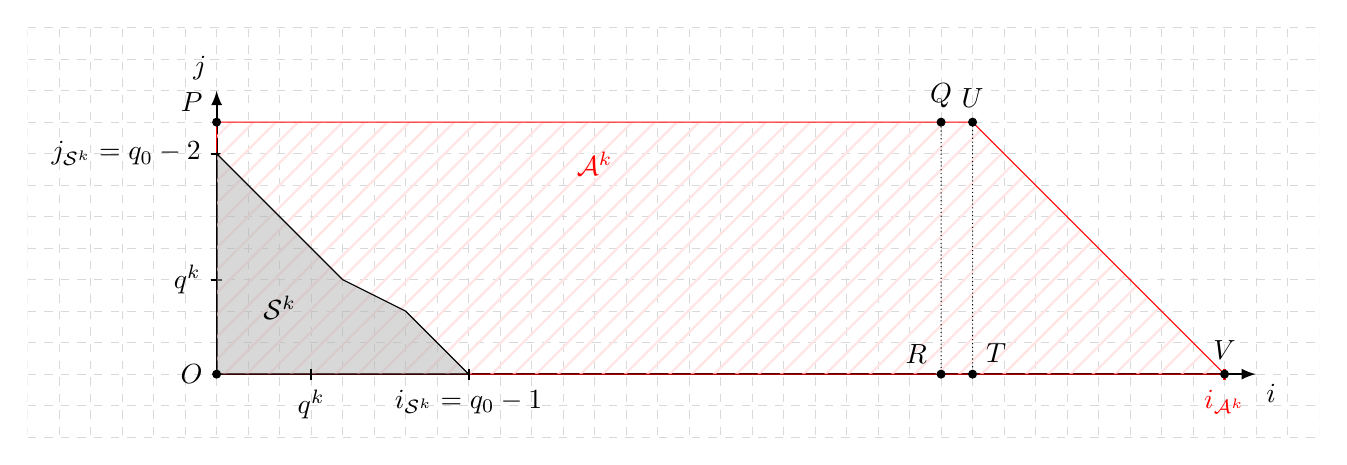
\begin{tikzpicture}[scale=0.4]
	\def\qO{9};
	\def\q{3};
	\pgfmathsetmacro\iAk{{(\qO-1)*(\q+1)}};
	\def\largeur{\iAk+3}
	\def\hauteur{\qO+2}
	\clip (-6,-2) rectangle (\largeur,\hauteur); % Clips the picture...
	\draw[style=help lines,dashed,opacity=0.3] (-6,-3) grid[step=1cm] (\largeur,\hauteur); % Draws a grid in the new coordinates.
	
	%Sommets des polygones
	%A^k
	\coordinate (O) at (0,0) {};
	\coordinate (V) at (\iAk,0) {};
	\coordinate (U) at (\iAk-\qO+1,\qO-1) {};
	\coordinate (P) at (0,\qO-1) {};
	%S^k
	\coordinate (D) at (\qO-1,0) {};
	\coordinate (E) at (\qO-3,2) {} ;
	\coordinate (F) at (\q+1,\q) {};
	\coordinate (G) at (0,\qO-2) {};
	
	
	
	%Marqueurs sur l'axe vertical
	\draw[thick] (5pt,\q) -- (-5pt,\q) node[anchor=east] {$q^k$} ;
	
	\draw[thick] (5pt,\qO-2) -- (-5pt,\qO-2) node[anchor=east] {$j_{\calS^k}=q_0-2$} ;
	
	
	%Axes
	\draw [thick,-latex] (0,0) -- (0,\qO) node [above left] {$j$};
	\draw [thick,-latex] (0,0) -- (\iAk+1,0) node [below right] {$i$};
		
	%Formes
	\filldraw [ pattern color=red!10,
	pattern={Lines[
		distance=2mm,
		angle=45,
		line width=0.3mm]},
	draw=red] (0,0) -- (V) -- (U) -- (P) -- cycle;
	
	\node[red,yshift=-1.5em] at ($(U)!0.5!(P)$) {$\calA^k$};
	
	
	
	\filldraw [fill=black!30, fill opacity=0.5, draw=black] ([c]0,0) -- ([c]D) -- ([c]E) -- ([c]F) -- ([c]G)-- cycle;
	
	\node[yshift=0.7em] at ($(0,0)!0.5!(F)$) {$\calS^k$};

	%Marqueurs sur l'axe horizontal
%\draw[thick,red] (\iAk-\qO+1,5pt) -- (\iAk-\qO+1,-5pt) node[anchor=north] {$i_{\calA^k}-(q_ 0-1)$} ;
\draw[thick,red] (\iAk,5pt) -- (\iAk,-5pt) node[anchor=north] {$i_{\calA^k}$} ;
\draw[thick] (\q,5pt) -- (\q,-5pt) node[anchor=north] {$q^k$} ;
\draw[thick] (\qO-1,5pt) -- (\qO-1,-5pt) node[anchor=north] {$i_{\calS^k}=q_0-1$} ;

	%Points

\node[draw,circle,inner sep=1pt,fill,black,label=180:$O$] at (O) {};		 		\node[draw,circle,inner sep=1pt,fill,black,label=170:$P$] at (P) {};
\node[draw,circle,inner sep=1pt,fill,black,label=90:$Q$] (Q) at ($(U)+(-1,0)$) {};
\node[draw,circle,inner sep=1pt,fill,black,label=170:$R$] (R) at ($(V)+(-\qO,0)$) {};
\node[draw,circle,inner sep=1pt,fill,black,label=30:$T$] (T) at  ($(V)+(-\qO+1,0)$) {};
\node[draw,circle,inner sep=1pt,fill,black,label=$U$] at (U) {};
\node[draw,circle,inner sep=1pt,fill,black,label=$V$] at (V) {};

\draw[densely dotted,] (Q) -- (R);	
\draw[densely dotted] (U) -- (T);	

	
\end{tikzpicture} }
	\caption{Case $2k \geq \frac{m}{2}$} \label{fig_case_2k>=m/2}
\end{figure}
\begin{figure}[ht] 
	\centering
	\scalebox{0.9}{
	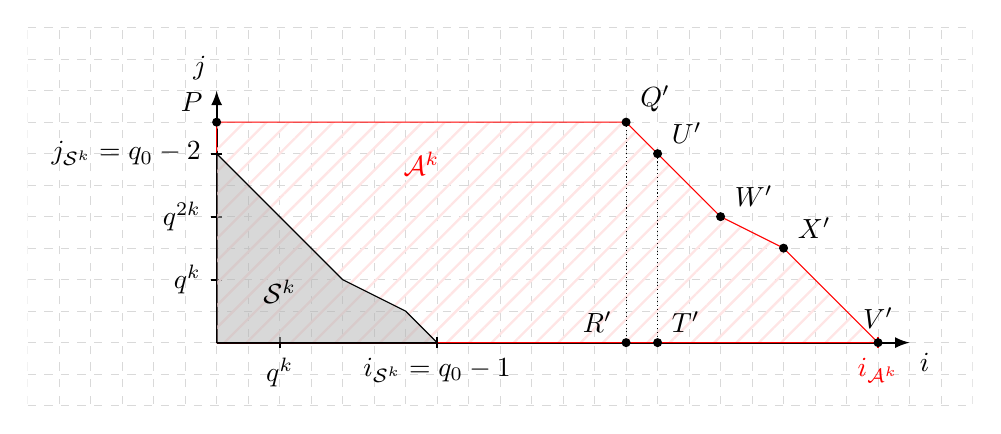
\begin{tikzpicture}[scale=0.4]
	\def\qO{8};
	\def\q{2};
	\def\iAk{21};
	\def\largeur{\iAk+3}
	\def\hauteur{\qO+2}
	\clip (-6,-2) rectangle (\largeur,\hauteur); % Clips the picture...
	\draw[style=help lines,dashed,opacity=0.3] (-6,-3) grid[step=1cm] (\largeur,\hauteur); % Draws a grid in the new coordinates.
	
	%Sommets des polygones
	\coordinate (A) at (\iAk,0) {};
	\coordinate (B) at (\iAk-\qO,\qO-1) {};
	\coordinate (C) at (0,\qO-1) {};
	\coordinate (D) at (0,\qO-2) {};
	\coordinate (E) at (\qO-1,0) {} ;
	\coordinate (F) at (2*\q,\q) {};
	\coordinate (G) at (\qO-2,1) {};
	\coordinate (H) at (18,3) {};
	\coordinate (I) at (16,4) {};
	
	
	%Marqueurs sur l'axe vertical
	\draw[thick] (5pt,\q) -- (-5pt,\q) node[anchor=east] {$q^k$} ;
	\draw[thick] (5pt,\qO-4) -- (-5pt,\qO-4) node[anchor=east] {$q^{2k}$} ;
	\draw[thick] (5pt,\qO-2) -- (-5pt,\qO-2) node[anchor=east] {$j_{\calS^k}=q_0-2$} ;
	
	
	%Marqueurs sur l'axe horizontal
	%\draw[thick,red] (\iAk-\qO,5pt) -- (\iAk-\qO,-5pt) node[anchor=north] {$i_{\calA^k}-q_ 0$} ;
	\draw[thick,red] (\iAk,5pt) -- (\iAk,-5pt) node[anchor=north] {$i_{\calA^k}$} ;
	\draw[thick] (\q,5pt) -- (\q,-5pt) node[anchor=north] {$q^k$} ;
	\draw[thick] (\qO-1,5pt) -- (\qO-1,-5pt) node[anchor=north] {$i_{\calS^k}=q_0-1$} ;
		
	%Axes
	\draw [thick,-latex] (0,0) -- (0,\qO) node [above left] {$j$};
	\draw [thick,-latex] (0,0) -- (\iAk+1,0) node [below right] {$i$};
	
	%Formes
	\filldraw [ pattern color=red!10,
	pattern={Lines[
		distance=2mm,
		angle=45,
		line width=0.3mm]},
	draw=red] (0,0) -- (A) -- (H) -- (I) -- (B) -- (C) -- cycle;
	
	\node[red,yshift=-1.5em] at ($(B)!0.5!(C)$) {$\calA^k$};
	
	
	\filldraw [fill=black!30, fill opacity=0.5, draw=black] ([c]0,0) -- ([c]E) -- ([c]G) -- ([c]F) -- ([c]D)-- cycle;
	
	\node[yshift=0.7em] at ($(0,0)!0.5!(F)$) {$\calS^k$};
	
	%Points du polygone
	\node[draw,circle,inner sep=1pt,fill,black,label=170:$P$] at (0,7) {};
	\node[draw,circle,inner sep=1pt,fill,black,label=3:$Q'$] at (13,7) {};
	\node[draw,circle,inner sep=1pt,fill,black,label=170:$R'$] at (13,0) {};
	\node[draw,circle,inner sep=1pt,fill,black,label=4:$T'$] at (14,0) {};
	\node[draw,circle,inner sep=1pt,fill,black,label=3:$U'$] at (14,6) {};
	\node[draw,circle,inner sep=1pt,fill,black,label=4:$W'$] at (16,4) {};
	\node[draw,circle,inner sep=1pt,fill,black,label=3:$X'$] at (18,3) {};
	\node[draw,circle,inner sep=1pt,fill,black,label=$V'$] at (21,0) {};
	
	\draw[densely dotted] (13,7) -- (13,0);	
	\draw[densely dotted] (14,6) -- (14,0);	
	
	
	
\end{tikzpicture} }
	\caption{Case $2k < \frac{m}{2}$} \label{fig_case_2k<m/2}
\end{figure}

 To prove that $\calA^k$ is included in $\calB^k$, we will use the partition above and prove that both parts are included in $\calB^k$. Let us first focus on the case where $2k \geq \frac{m}{2}$.



%We will prove first it the case $2k \geq \frac{m}{2}$, similar arguments works \modifier{for the other one}. Taking a point $b(i_b,j_b)$ in $\calA^k$, we can distinguish two cases:

\begin{itemize}
\item To prove that $\Gamma \subset \calB^k$, we will fix an abscissa $i$ of a point in $\Gamma$ and we will show that all points $(i,0),\cdots,(i,q_0-1)$ belong to $\calB^k$. By definition of $\Gamma$, we have $i < i_{\calS^k}q^k=(q_0-1)q^k$. Let us write
    \[i = \alpha q^k+\gamma \text{ with } \alpha <q_0-1 \text{ and } \gamma < q^k.\]
   
   	Set $j^*:=\max \{j \ | \ (\alpha,j) \in \calS^k\} = \left\lfloor \frac{s-\alpha q_0}{q_0+1}\right\rfloor$. This is well--defined because $\alpha \leq q_0 -2$ and $j^*$ is at least equal to $1$. We will show that the integral points on the vertical line of abscissa $i$ belong to $B^k$, and more precisely that
    \[\left\{ (i,0),\cdots,(i,q_0-1) \right\} \subset \bigcup_{j=0}^{j^*} \calS^k_{(\alpha,j)}.\]
    Let $0 \leq j \leq j^*$. Then the point $(\alpha,j)$ belongs to $\calS^k$. Moreover for every $0 \leq r \leq q_0-2-\gamma$ the point $(i,jq^k+r)=q^k(\alpha,j)+(\gamma,r)$ lies in the set $\calS^k_{(\alpha,j)}$.
     
    Let us check that $\min \{y \mid (i,y) \in \calS^k_{(\alpha,j+1)} \} \leq \max \{y \mid (i,y) \in \calS^k_{(\alpha,j)}\}+1$, in which case we have
    
    \begin{equation}\label{eq:ligne_verticale}\left\{ (i,0),\cdots,(i,j^*q^k+q_0-2-\gamma) \right\} \subset \bigcup_{j=0}^{j^*} \calS^k_{(\alpha,j)}.
    \end{equation}
	One can easily check that    
    \begin{align*}
    	\min \{y \mid (i,y) \in \calS^k_{(\alpha,j+1)} \} & =     (j+1)q^k, \\
    	\max \{y \mid (i,y) \in \calS^k_{(\alpha,j)}\} & = jq^k + (q_0-2-\gamma)
    \end{align*}
	and we have the desired inequality, reached for $q^k=q=2$ and $q_0=4$. As $j^* \geq 1$ and $\gamma < q^k$, the maximal ordinate $j^*q^k+q_0-2-\gamma$ in \eqref{eq:ligne_verticale} is larger than or equal to $q_0-1$, which concludes this part of the proof.
	
	
	%Now, it remains to prove that $j^*q^k+q_0-2-\gamma \geq q_0-1$.    The minimal value of $j^*$ is attained when $\alpha = q_0-2$ is maximal. In this situation, we have 
    %\[j^* = \left\lfloor \dfrac{q_0+q^k-1}{q_0+1}\right\rfloor \geq 1,\]
    %and $q^k+q_0-2-\gamma \geq q_0-1$, since $\gamma < q^k$. 
    
    \mathieu{Est-ce qu'on garde la Figure 3? j'ai décalé les petits triangles au max du bords droit du triangle.} \jade{Oui, j'aime bien :)}



\begin{figure}[ht]
\centering
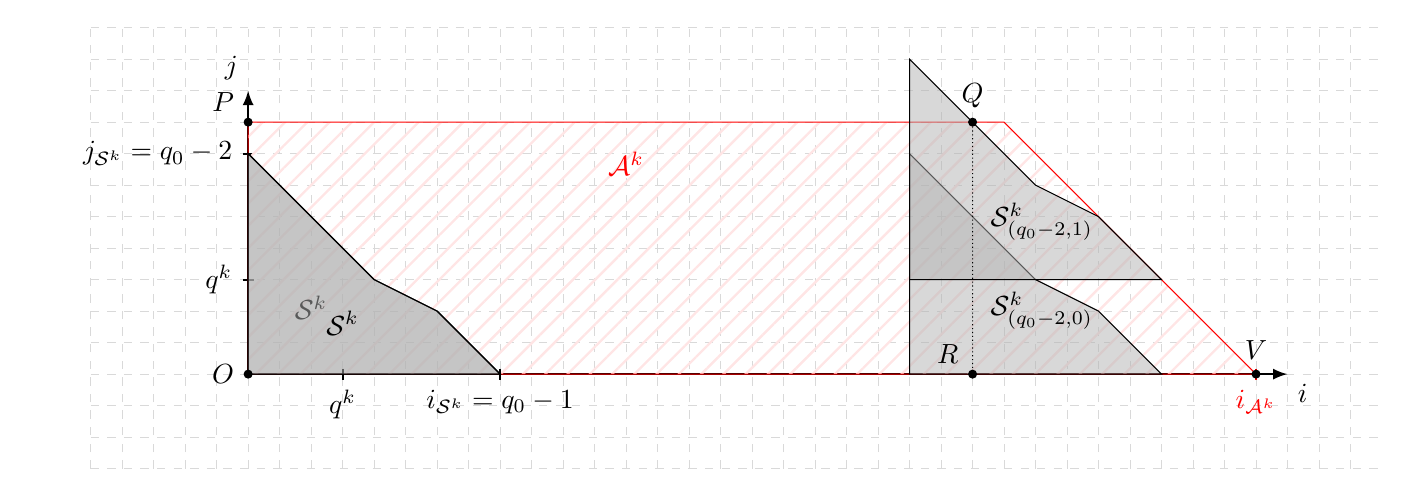
\begin{tikzpicture}[scale=0.4]
	
	\def\qO{9};
	\def\q{3};
	\def\iAk{32};
	\def\largeur{\iAk+4}
	\def\hauteur{\qO+2}
	\clip (-7,-3) rectangle (\largeur,\hauteur); % Clips the picture...
	\draw[style=help lines,dashed,opacity=0.3] (-5,-3) grid[step=1cm] (\largeur,\hauteur); % Draws a grid in the new coordinates.
	
	%Sommets des polygones
	%A^k
	\coordinate (O) at (0,0) {};
	\coordinate (V) at (\iAk,0) {};
	\coordinate (U) at (\iAk-\qO+1,\qO-1) {};
	\coordinate (P) at (0,\qO-1) {};
	%S^k
	\coordinate (D) at (\qO-1,0) {};
	\coordinate (E) at (\qO-3,2) {} ;
	\coordinate (F) at (\q+1,\q) {};
	\coordinate (G) at (0,\qO-2) {};
	
	
	
	%Marqueurs sur l'axe vertical
	\draw[thick] (5pt,\q) -- (-5pt,\q) node[anchor=east] {$q^k$} ;
	
	\draw[thick] (5pt,\qO-2) -- (-5pt,\qO-2) node[anchor=east] {$j_{\calS^k}=q_0-2$} ;
	
	
	%Axes
	\draw [thick,-latex] (0,0) -- (0,\qO) node [above left] {$j$};
	\draw [thick,-latex] (0,0) -- (\iAk+1,0) node [below right] {$i$};
	
	%Formes
	\filldraw [ pattern color=red!10,
	pattern={Lines[
		distance=2mm,
		angle=45,
		line width=0.3mm]},
	draw=red] (0,0) -- (V) -- (U) -- (P) -- cycle;
	
	\node[red,yshift=-1.5em] at ($(U)!0.5!(P)$) {$\calA^k$};
	
	
	
	\filldraw [fill=black!30, fill opacity=0.5, draw=black] ([c]0,0) -- ([c]D) -- ([c]E) -- ([c]F) -- ([c]G)-- cycle;
	
	\node[yshift=0.7em] at ($(0,0)!0.5!(F)$) {$\calS^k$};
	
	%Marqueurs sur l'axe horizontal
	%	\draw[thick,red] (\iAk-\qO+1,5pt) -- (\iAk-\qO+1,-5pt) node[anchor=north] {$i_{\calA^k}-(q_ 0-1)$} ;
	\draw[thick,red] (\iAk,5pt) -- (\iAk,-5pt) node[anchor=north] {$i_{\calA^k}$} ;
	\draw[thick] (\q,5pt) -- (\q,-5pt) node[anchor=north] {$q^k$} ;
	\draw[thick] (\qO-1,5pt) -- (\qO-1,-5pt) node[anchor=north] {$i_{\calS^k}=q_0-1$} ;
	
	
	\foreach \coord in{(0,0),({\q*(\qO-2)},0),({\q*(\qO-2)},\q)} {
		\begin{scope}[every coordinate/.style={shift={\coord}}]
			\filldraw [fill=black!30, fill opacity=0.5, draw=black] ([c]0,0) -- ([c]D) -- ([c]E) -- ([c]F) -- ([c]G)-- cycle;
		\end{scope}
	}
	
	
	
	%Points
	
	\node[draw,circle,inner sep=1pt,fill,black,label=180:$O$] at (O) {};		 		\node[draw,circle,inner sep=1pt,fill,black,label=170:$P$] at (P) {};
	\node[draw,circle,inner sep=1pt,fill,black,label=90:$Q$] (Q) at ($(U)+(-1,0)$) {};
	\node[draw,circle,inner sep=1pt,fill,black,label=170:$R$] (R) at ($(V)+(-\qO,0)$) {};
	%	\node[draw,circle,inner sep=1pt,fill,black,label=30:$T$] (T) at  ($(V)+(-\qO+1,0)$) {};
	%	\node[draw,circle,inner sep=1pt,fill,black,label=$U$] at (U) {};
	\node[draw,circle,inner sep=1pt,fill,black,label=$V$] at (V) {};
	
	\draw[densely dotted,] (Q) -- (R);	
	%	\draw[densely dotted] (U) -- (T);	
	
	
	
	\node[yshift=0.7em] at ($(0,0)!0.5!(E)$) {$\calS^k$};
	\node[yshift=0.7em] at ($(0,0)!0.7!(E)+({\q*(\qO-2)},0)$) {$\calS^k_{(q_0-2,0)}$};
	\node[yshift=0.5em] at ($(0,0)!0.7!(E)+({\q*(\qO-2)},\q)$) {$\calS^k_{(q_0-2,1)}$};
	
	
	
	
\end{tikzpicture} 
\caption{Example with $2k \geq \frac{m}{2}$ and $i \leq (q_0-1)q^k$} \label{ex_in_rectangle}
\end{figure}

 \item[$\star$] Now let us prove $\Delta \subset \calB^k$. First note that for every $\delta \in \{0,..,q^k-1\}$, we have $(i_{\calS^k}-\delta,\delta) \in \calS^k$, as 
  \[q_0(i_{\calS^k}-\delta) + \delta(q_0+1) = q_0(q_0-1)+\delta-1 \leq s.\]
 
 We aim to prove
 \begin{equation} \label{eq:Delta_Bigcup}
 \Delta \subseteq \bigcup_{\delta=0}^{q^k-1} \calS^k_{(i_{\calS^k}-\delta,\delta)}.
 \end{equation}
\modifier{See the Figure \ref{ex_in_triangle} to compare $\Delta$ and $\bigcup_{\delta=0}^{q^k-1} \calS^k_{(i_{\calS^k}-\delta,\delta)}$ on a example.}
\mathieu{il reste des trucs à modifier sur la Figure 4?}

By definition $\Delta = \calA^k \cap \left\{(i,j)\in \Z^2 \mid i \geq i_{\calS^k}q^k\right\}$ and $\calS^k_{(i_{\calS^k},0)}=q^k(i_{\calS^k},0)+\calS^k$.
Therefore, to verify that $\calS^k_{(i_{\calS^k},0)} \subset \Delta$, it is enough to check that $\calS^k_{(i_{\calS^k},0)} \subset \calA^k$. This follows from the following inequality:
\[\forall \: (i_0,j_0) \in \calS^k, \: (i_{\calS^k}q^k+i_0)q_0+j_0(q_0+1)\leq i_{\calS^k}q^kq_0+s \leq s(q^k+1).\]
To prove \eqref{eq:Delta_Bigcup}, it remains to check that the each point
$\Delta \setminus  \calS^k_{(i_{\calS^k},0)}$ lies in some $\calS^k_{(i_{\calS^k}-\delta,\delta)}$ for $\delta\geq 1$.

Let us compute the cardinality of $\Delta \setminus  \calS^k_{(i_{\calS^k},0)}$. A short calculation gives
 \[ \# \Delta = \dfrac{q_0(q_0+1)}{2} \quad \mathrm{and} \quad \# \calS^k_{(i_{\calS^k},0)} = \dim \calL(sP_{\infty}) = s+1-g(\calH) = \dfrac{q_0(q_0-1)}{2} + q^k.\]

Then $\# \Delta \setminus  \calS^k_{(i_{\calS^k},0)}=q_0-q^k$. Besides, one can easily check that the $q_0-q^k$ points of coordinates $(i_{\calA^k}-\mu,\mu)$ for $q^k \leq \mu \leq q_0-1$ cannot be in $\calS^k_{(i_{\calS^k},0)}$, as $(i_{\calS^k}-\mu,\mu) \notin \calS^k$. Then $\Delta \setminus  \calS^k_{(i_{\calS^k},0)}$ contains exactly these points, and no other. Writing
 \[ \mu = \mu_1q^k + \mu_2,\]
 with $\mu_2 < q^k$ and $1 \leq \mu_1 \leq \left\lfloor\frac{q_0-1}{q^k}\right\rfloor \leq q^{m/2-k}-1 \leq q^k-1$ (since $k \geq m/4$). One can easily deduce that
 \[(i_{\calA^k}-\mu,\mu)=q^k(i_{\calS^k}-\mu_1,\mu_1)+(i_{\calS^k}-\mu_2,\mu_2) \in \calS^k_{i_{\calS^k}-\mu_1,\mu_1},\]
 which entails the inclusion \eqref{eq:Delta_Bigcup}.
% Note that $q^k$ of these points are in $\calS^k_{((q_0-1),0)})$ (case $\mu_1=0)$, meaning that the remaining $q_0-q^k$ are in $(\Delta \backslash  \calS^k_{((q_0-1),0)})$, which proves \eqref{counting}


 
\begin{figure}[ht]
\centering
	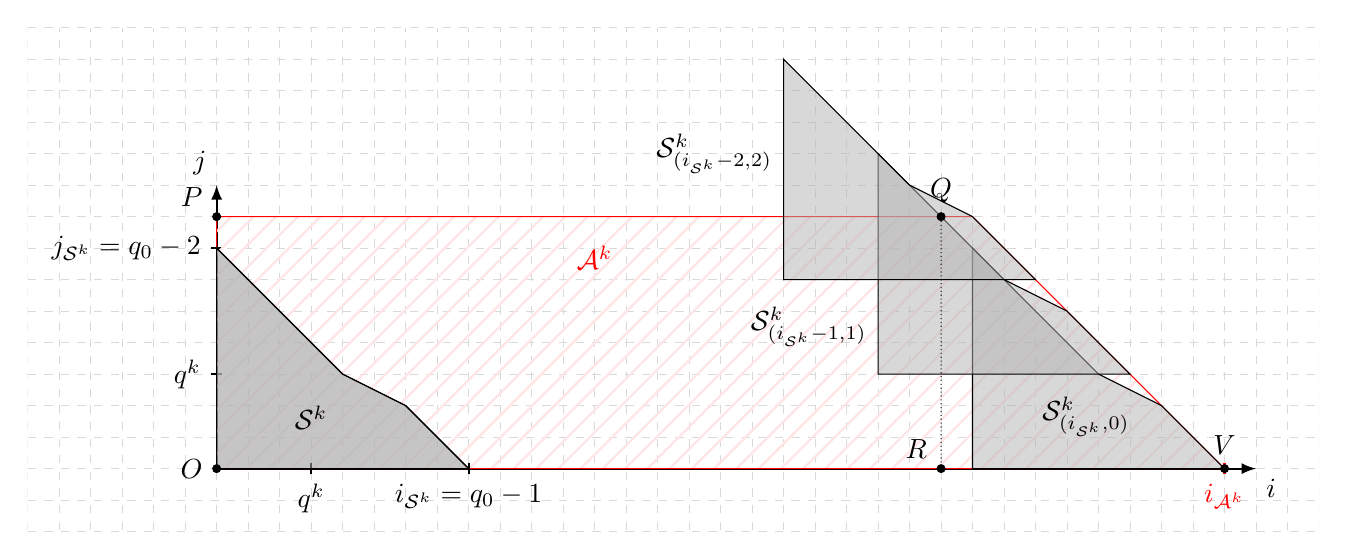
\begin{tikzpicture}[scale=0.4]
	
	\def\qO{9};
	\def\q{3};
	\def\iAk{32};
	\def\largeur{\iAk+3}
	\def\hauteur{\qO+5}
	\clip (-6,-2) rectangle (\largeur,\hauteur); % Clips the picture...
	\draw[style=help lines,dashed,opacity=0.3] (-6,-3) grid[step=1cm] (\largeur,\hauteur); % Draws a grid in the new coordinates.
	
	%Sommets des polygones
	%A^k
	\coordinate (O) at (0,0) {};
	\coordinate (V) at (\iAk,0) {};
	\coordinate (U) at (\iAk-\qO+1,\qO-1) {};
	\coordinate (P) at (0,\qO-1) {};
	%S^k
	\coordinate (D) at (\qO-1,0) {};
	\coordinate (E) at (\qO-3,2) {} ;
	\coordinate (F) at (\q+1,\q) {};
	\coordinate (G) at (0,\qO-2) {};
	
	
	
	%Marqueurs sur l'axe vertical
	\draw[thick] (5pt,\q) -- (-5pt,\q) node[anchor=east] {$q^k$} ;
	
	\draw[thick] (5pt,\qO-2) -- (-5pt,\qO-2) node[anchor=east] {$j_{\calS^k}=q_0-2$} ;
	
	
	%Axes
	\draw [thick,-latex] (0,0) -- (0,\qO) node [above left] {$j$};
	\draw [thick,-latex] (0,0) -- (\iAk+1,0) node [below right] {$i$};
	
	%Formes
	\filldraw [ pattern color=red!10,
	pattern={Lines[
		distance=2mm,
		angle=45,
		line width=0.3mm]},
	draw=red] (0,0) -- (V) -- (U) -- (P) -- cycle;
	
	\node[red,yshift=-1.5em] at ($(U)!0.5!(P)$) {$\calA^k$};
	
	
	
	\filldraw [fill=black!30, fill opacity=0.5, draw=black] ([c]0,0) -- ([c]D) -- ([c]E) -- ([c]F) -- ([c]G)-- cycle;
		
	%Marqueurs sur l'axe horizontal
	%	\draw[thick,red] (\iAk-\qO+1,5pt) -- (\iAk-\qO+1,-5pt) node[anchor=north] {$i_{\calA^k}-(q_ 0-1)$} ;
	\draw[thick,red] (\iAk,5pt) -- (\iAk,-5pt) node[anchor=north] {$i_{\calA^k}$} ;
	\draw[thick] (\q,5pt) -- (\q,-5pt) node[anchor=north] {$q^k$} ;
	\draw[thick] (\qO-1,5pt) -- (\qO-1,-5pt) node[anchor=north] {$i_{\calS^k}=q_0-1$} ;
	
	\foreach \coord in{(0,0),(\iAk-\qO+1,0),(\iAk-\qO+1-\q,\q),(\iAk-\qO+1-2*\q,2*\q)} {
	\begin{scope}[every coordinate/.style={shift={\coord}}]
		\filldraw [fill=black!30, fill opacity=0.5, draw=black] ([c]0,0) -- ([c]D) -- ([c]E) -- ([c]F) -- ([c]G)-- cycle;
	\end{scope}
}
	
	
	%Points
	
	\node[draw,circle,inner sep=1pt,fill,black,label=180:$O$] at (O) {};		 		\node[draw,circle,inner sep=1pt,fill,black,label=170:$P$] at (P) {};
	\node[draw,circle,inner sep=1pt,fill,black,label=90:$Q$] (Q) at ($(U)+(-1,0)$) {};
	\node[draw,circle,inner sep=1pt,fill,black,label=170:$R$] (R) at ($(V)+(-\qO,0)$) {};
	%	\node[draw,circle,inner sep=1pt,fill,black,label=30:$T$] (T) at  ($(V)+(-\qO+1,0)$) {};
	%	\node[draw,circle,inner sep=1pt,fill,black,label=$U$] at (U) {};
	\node[draw,circle,inner sep=1pt,fill,black,label=$V$] at (V) {};
	
	\draw[densely dotted,] (Q) -- (R);	
	%	\draw[densely dotted] (U) -- (T);	
	
	
	


	


\node[yshift=0.7em] at ($(0,0)!0.5!(E)$) {$\calS^k$};
\node[yshift=0.5em] at ($(0,0)!0.6!(E)+({\q*(\qO-1)},0)$) {$\calS^k_{(i_{\calS^k},0)}$};
\node at ($(-2.2,1.5)+({\q*(\qO-2)},\q)$) {$\calS^k_{(i_{\calS^k}-1,1)}$};
\node at ($(-2.2,4)+({\q*(\qO-3)},2*\q)$) {$\calS^k_{(i_{\calS^k}-2,2)}$};

	
\end{tikzpicture} 
\caption{Example with $2k \geq \frac{m}{2}$ and $i \geq (q_0-1)q^k$} \label{ex_in_triangle}

\end{figure}
\end{itemize}

Now let us deal with the case $2k < \frac{m}{2}$. The proof for the inclusion $\Gamma' \subset \calB^k$ is almost identical to the one for $\Gamma \subset \calB^k$ in the previous case.

Let us prove that $\Delta' \subset \calB^k$. As before, for every $\delta \in \{0,..,q^k-1\}$, we have $(i_{\calS^k}-\delta,\delta) \in \calS^k$, and we aim to prove
\begin{equation} \label{eq:Delta'_Bigcup}
	\Delta' \subseteq \bigcup_{\delta=0}^{q^k-1} \calS^k_{(i_{\calS^k}-\delta,\delta)}.
\end{equation}
Similarly, we have $\calS^k_{(i_{\calS^k},0)} \subset \Delta'$. Thus, in order to prove \eqref{eq:Delta'_Bigcup}, it remains to check that the each point
$\Delta \setminus  \calS^k_{(i_{\calS^k},0)}$ lies in some $\calS^k_{(i_{\calS^k}-\delta,\delta)}$ for $\delta\geq 1$.

In this case, $ \# \Gamma = \dfrac{q_0(q_0-1)}{2}+q^{2k}$, and thus $\# (\Gamma \backslash  \calS^k_{(q_0-1,0)}) = q^{2k}-q^k$. As in the previous case, we are able to determine these $q^{2k}-q^k$ points. These are the ones of the form
\[ (i_{\calA^k}-\mu,\mu) \ , \ \mathrm{where} \ \mu \in \{q^k,\cdots,q^{2k}-1\},\]
which lie on the path joining $U'$ and $V'$. 
For every $\mu \in \{q^k,\cdots,q^{2k}-1\}$, we write $\mu = \mu_1 q^k + \mu_2 \ , \ \mathrm{with} \ \mu_1,\mu_2 < q^k$ and we claim  \[(i_{\calA^k}-\mu,\mu)=q^k(i_{\calS^k}-\mu_1,\mu_1)+(i_{\calS^k}-\mu_2,\mu_2) \in \calS^k_{i_{\calS^k}-\mu_1,\mu_1},\]
which proves \eqref{eq:Delta'_Bigcup} and completes the proof.
\mathieu{Figure \ref{ex_polygone} below show an example in this case.}

\begin{figure}[ht]
\begin{center}
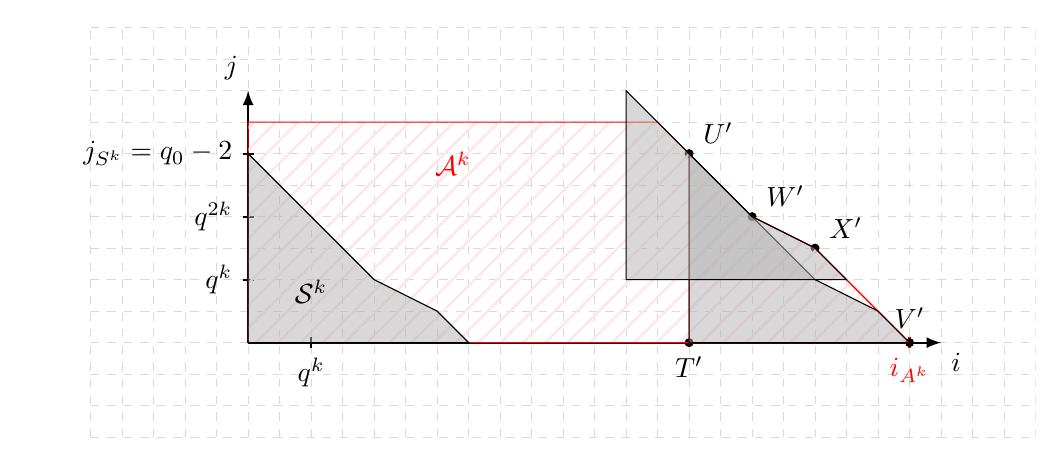
\begin{tikzpicture}[scale=0.4]
	\def\qO{8};
	\def\q{2};
	\def\iAk{21};
	\def\largeur{\iAk+4}
	\def\hauteur{\qO+2}
\clip (-7,-3) rectangle (\largeur,\hauteur); % Clips the picture...
\draw[style=help lines,dashed,opacity=0.3] (-5,-3) grid[step=1cm] (\largeur,\hauteur); % Draws a grid in the new coordinates.

%Sommets des polygones
\coordinate (A) at (\iAk,0) {};
\coordinate (B) at (\iAk-\qO,\qO-1) {};
\coordinate (C) at (0,\qO-1) {};
\coordinate (D) at (0,\qO-2) {};
\coordinate (E) at (\qO-1,0) {} ;
\coordinate (F) at (2*\q,\q) {};
\coordinate (G) at (\qO-2,1) {};
\coordinate (H) at (18,3) {};
\coordinate (I) at (16,4) {};


%Marqueurs sur l'axe vertical
\draw[thick] (5pt,\q) -- (-5pt,\q) node[anchor=east] {$q^k$} ;
\draw[thick] (5pt,\qO-4) -- (-5pt,\qO-4) node[anchor=east] {$q^{2k}$} ;
\draw[thick] (5pt,\qO-2) -- (-5pt,\qO-2) node[anchor=east] {$j_{S^k}=q_0-2$} ;


%Marqueurs sur l'axe horizontal
%\draw[thick,red] (\iAk-\qO,5pt) -- (\iAk-\qO,-5pt) node[anchor=north] {$i_{A^k}-q_ 0$} ;
\draw[thick,red] (\iAk,5pt) -- (\iAk,-5pt) node[anchor=north] {$i_{A^k}$} ;
\draw[thick] (\q,5pt) -- (\q,-5pt) node[anchor=north] {$q^k$} ;
%\draw[thick] (\qO-1,5pt) -- (\qO-1,-5pt) node[anchor=north] {$i_{S^k}=q_0-1$} ;



%Axes
\draw [thick,-latex] (0,0) -- (0,\qO) node [above left] {$j$};
\draw [thick,-latex] (0,0) -- (\iAk+1,0) node [below right] {$i$};

%Points du polygone
\node[draw,circle,inner sep=1pt,fill,black,label=270:$T'$] at (14,0) {};
\node[draw,circle,inner sep=1pt,fill,black,label=3:$U'$] at (14,6) {};
\node[draw,circle,inner sep=1pt,fill,black,label=4:$W'$] at (16,4) {};
\node[draw,circle,inner sep=1pt,fill,black,label=3:$X'$] at (18,3) {};
\node[draw,circle,inner sep=1pt,fill,black,label=$V'$] at (21,0) {};



%Formes
\filldraw [ pattern color=red!10,
	pattern={Lines[
	distance=2mm,
	angle=45,
	line width=0.3mm]},
	draw=red] (0,0) -- (A) -- (H) -- (I) -- (B) -- (C) -- cycle;
	
\filldraw [ pattern color=red!10,
	pattern={Lines[
	distance=2mm,
	angle=45,
	line width=0.3mm]},
	draw=red] (14,0) -- (21,0) -- (18,3) -- (16,4) -- (14,6)  -- cycle;
	
\filldraw[fill=black!30, fill opacity=0.5, draw=black] (14,0) -- (21,0) -- (20,1) -- (18,2) -- (14,6)  -- cycle;

\filldraw[fill=black!30, fill opacity=0.5, draw=black] (12,2) -- (19,2) -- (18,3) -- (16,4) -- (12,8)  -- cycle;
	
\node[red,yshift=-1.5em] at ($(B)!0.5!(C)$) {$\calA^k$};


\filldraw [fill=black!30, fill opacity=0.5, draw=black] ([c]0,0) -- ([c]E) -- ([c]G) -- ([c]F) -- ([c]D)-- cycle;

	\node[yshift=0.7em] at ($(0,0)!0.5!(F)$) {$\calS^k$};

 
\end{tikzpicture} 
\caption{Example with $2k < \frac{m}{2}$ and $i \geq q^k(q_0-1)$} \label{ex_polygone}
\end{center}
\end{figure}

\end{proof}


\begin{rq1} 
In the picture below, you can find a counter-example in the case $\calB^k \ne \calA^k$ if $s$ does not reach the bound given in Proposition \ref{prop_avec_dessins}. \jade{Here, with $s=\mu_g+q^k-1$, we can see that some monomials $x^iy^j \in \calL((q+1)sP_\infty)$ cannot be written as a product $x^{i_1+qi_2}y^{j_1+qj_2}$ for $(i_r,j_r) \in \calS_k$.}
	\begin{figure}[ht]
		\begin{center}
			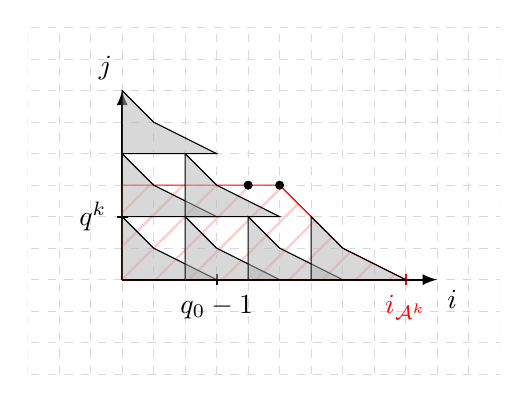
\begin{tikzpicture}[scale=0.4]
				\def\qO{4};
				\def\q{2};
				\def\iAk{9};
				\def\largeur{\iAk+3}
				\def\hauteur{\qO+4}
				\clip (-3,-3) rectangle (\largeur,\hauteur); % Clips the picture...
				\draw[style=help lines,dashed,opacity=0.3] (-5,-3) grid[step=1cm] (\largeur,\hauteur); % Draws a grid in the new coordinates.
				
				%Sommets des polygones
				%A^k
				\coordinate (A) at (\iAk,0) {};
				\coordinate (B) at (\iAk-\qO,\qO-1) {};
				\coordinate (C) at (0,\qO-1) {};
				%S^k
				\coordinate (D) at (\qO-1,0) {};
				\coordinate (E) at (\qO-3,2) {} ;
				\coordinate (F) at (\q+1,\q) {};
				\coordinate (G) at (0,\qO-2) {};
				
				
				%finir le rectangle
				\coordinate (H) at (\iAk-\qO,0) {};
				
				
				%Marqueurs sur l'axe vertical
				\draw[thick] (5pt,\q) -- (-5pt,\q) node[anchor=east] {$q^k$} ;
				%\draw[thick] (5pt,\qO-4) -- (-5pt,\qO-4) node[anchor=east] {$q^{2k}$} ;
				
				
				
				%Marqueurs sur l'axe horizontal
				%\draw[thick,red] (\iAk-\qO+1,5pt) -- (\iAk-\qO+1,-5pt) node[anchor=north] {$i_{\calA^k}-(q_ 0-1)$} ;
				\draw[thick,red] (\iAk,5pt) -- (\iAk,-5pt) node[anchor=north] {$i_{\calA^k}$} ;
				% \draw[thick] (\q,5pt) -- (\q,-5pt) node[anchor=north] {$q^k$} ;
				\draw[thick] (\qO-1,5pt) -- (\qO-1,-5pt) node[anchor=north] {$q_0-1$} ;
				
				
				
				%Axes
				\draw [thick,-latex] (0,0) -- (0,\qO+2) node [above left] {$j$};
				\draw [thick,-latex] (0,0) -- (\iAk+1,0) node [below right] {$i$};
				
				%Formes
				\filldraw [ pattern color=red!20,
				pattern={Lines[
					distance=3mm,
					angle=45,
					line width=0.3mm]},
				draw=red] (0,0) -- (9,0) -- (7,1) -- (5,3) -- (0,3)-- cycle;
				
				\foreach \i in {0,1,2,3}{
					\filldraw [fill=black!30, fill opacity=0.5, draw=black] (2*\i,0) -- (3+2*\i,0) -- (1+2*\i,1) -- (2*\i,2)-- cycle;
				}
				
				\foreach \i in {0,1}{
					\filldraw [fill=black!30, fill opacity=0.5, draw=black] (2*\i,2) -- (3+2*\i,2) -- (1+2*\i,3) -- (2*\i,4)-- cycle;
				}
				
				\filldraw [fill=black!30, fill opacity=0.5, draw=black] (0,4) -- (3,4) -- (1,5) -- (0,6)-- cycle;
				
				\node[draw,circle,inner sep=1pt,fill,black] at (4,3) {};
				\node[draw,circle,inner sep=1pt,fill,black] at (5,3) {};
				
				
				
			\end{tikzpicture} 
		\end{center}
		\caption{Counter-example with $(q,q_0,s,k)= (2,4,1,\mu_g+q-1)$}
		
	\end{figure}
\end{rq1}




\newpage


































\begin{rq1}
The difference between Propositions \ref{prop:result_with_valuations_case_q0} and \ref{prop:powers_of_q's_case} is that in the second case, we are only able to give a sufficient condition.
\end{rq1} 

From this two results, we deduce:

\begin{coro1} \label{coro:_inclusion_code_SSAG_case}
Let $\calC = C_{\calL}(\calH,\calP,sP_{\infty})$ be the AG-code on $\calH$ over $\mathbb{F}_{q^m}=\mathbb{F}_{q_0^2}$ associated to a support $\calP \subseteq\calH(\F_{q_0^2})\setminus \{P_{\infty}\}$ and to the one-point divisor $sP_{\infty}$. Denote by $g:=g(\calH)=\frac{q_0(q_0-1)}{2}$ and $\mu_g := q_0(q_0-1)-1$ the biggest gap number of $P_{\infty}$. 
\begin{itemize}
    \item[(i)] If $s \geq \mu_g + q_0^2$, then we have 
        \[\Tr{\calC \star \calC} \subseteq \Tr{\calC \star \calC^q} \subseteq \cdots \subseteq \Tr{\calC \star \calC^{q_0}},\]
        and thus 
        \[\Tr{\calC}^{\star 2} \subseteq \Tr{\calC \star \calC^{q_0}}.\]
    \item[(ii)] If $\mu_g < s < \mu_g +q_0^2$, denote by $f:= \max\set{k \in \{0,\cdots,\frac{m}{2}-1\} : s \geq \mu_g + q^k}$ \jade{$=\log_q\Floor{s-\mu_g}$ serait plus simple, non ?}. In this case, we have 
        \[\Tr{\calC \star \calC} \subseteq \Tr{\calC \star \calC^q} \subseteq \cdots \subseteq \Tr{\calC \star \calC^{q^f}},\]
          and then
        \[\Tr{\calC}^{\star 2} \subseteq \Tr{\calC \star \calC^{q^f}} + \sum\limits_{i=f+1}^{m/2} \Tr{\calC \star \calC^{q^i}}.\]
\end{itemize}
\end{coro1}

\begin{proof}
$(i)$ is a consequence of Proposition \ref{prop:result_with_valuations_case_q0} in the case $i=1$ (note that the result also holds without the Trace operator), while $(ii)$ uses Proposition \ref{prop:powers_of_q's_case} several times. In both cases, we get a result on $\Tr{\calC}^{\star 2}$ by using Theorem \ref{th:Tr_BoundSchurSquare}.
\end{proof}

Using the above Corollary and Lemma \ref{lem:known_bounds}, we can prove the following theorem, that gives an upperbound on the dimension of the trace of the square of the dual of our one-point Hermitian SSAG-code which can be compared to the one given in Corollary \ref{square_ssag_bound}.

\begin{thm} \label{th:our_sup_bounds_on_codes}
We keep notations as in Corollary \ref{coro:_inclusion_code_SSAG_case}, and denote by $k$ the dimension of $\calC$ over $\fqm$.
\begin{itemize}
\item[(i)] If $s \geq \mu_g + q_0^2$, then 
\[   \dim_{\fq} \Tr{\calC}^{\star 2}  \leq \binom{mk+1}{2} - \dfrac{m}{2} (k(mk-1)-2q_0s).\]
\item[(ii)] If $\mu_g < s < \mu_g +q_0^2$, recall that $f:= \max\{k \in \{0,\cdots,\frac{m}{2}-1\} : s \geq \mu_g + q^k\}$ \jade{idem}. Then 
\[   \dim_{\fq} \Tr{\calC}^{\star 2}  \leq \binom{mk+1}{2} - \dfrac{m}{2}(k(2fk-1)-2q^fs).\]
\end{itemize}
\end{thm}

\begin{proof}
\begin{itemize}
    \item[$(i)$] From \ref{coro:_inclusion_code_SSAG_case} $(i)$, we have $\Tr{\calC}^{\star 2} \subseteq \Tr{\calC \star \calC^{q_0}}.$ Moreover, we proved in Proposition \ref{prop:result_with_valuations_case_q0} that under the hypothesis on $s$, we had
      \[ \calC \star \calC^{q_0} = \calC^{\star (q_0+1)} := C_{\calL}(\calH,\calP,(q_0+1)sP_{\infty}),\]
      which has dimension $(q_0+1)s + 1 - g(\calH)$ by the Riemann-Roch theorem. As a result, we can estimate
      \begin{align*}
           \dim_{\fq} \Tr{\calC}^{\star 2} &\leq \dim_{\fq} \Tr{\calC^{\star (q_0+1)}} \\
                                            & = m((q_0+1)s + 1 - g(\calH)) \jade{\text{pk une égalité ici ?}}\\
                                            & = m (k+q_0 s) \\
                                            & = \binom{mk+1}{2} + \dfrac{m}{2}(2k+2q_0s-k(mk+1)) \\
                                            &= \binom{mk+1}{2} - \dfrac{m}{2} (k(mk-1)-2q_0s).
      \end{align*}
      \item[$(ii)$] \ref{coro:_inclusion_code_SSAG_case} $(ii)$ together with Proposition \ref{prop:powers_of_q's_case} gives 
       \[\Tr{\calC}^{\star 2} \subseteq \Tr{\calC \star \calC^{q^f}} + \sum\limits_{i=f+1}^{m/2} \Tr{\calC \star \calC^{q^i}}\]
       and 
        \[ \calC \star \calC^{q^f} = \calC^{q^f+1} := C_{\calL}(\calH,\calP,(q^f+1)sP_{\infty}).\]
        Since the latter code has dimension $(q^f+1)s+1-g(\calH)=k+q^fs$, we have (using twice Lemma \ref{lem:known_bounds})
         \begin{align*}
           \dim_{\fq}\Tr{\calC}^{\star 2} &\leq \dim_{\fq}\Tr{\calC^{\star(q_f+1)}} +  \sum\limits_{i=f+1}^{m/2} \dim_{\fq} \Tr{\calC \star \calC^{q^i}}\\
                                            &\leq m \cdot (k + q^fs) + m  \sum\limits_{i=f+1}^{m/2} \dim_{\fqm}(\calC \star \calC^{q^i}) \\
                                            &\leq m \cdot \left(k+q^fs + k^2 \left(\frac{m}{2}-f\right)\right). \\
                                            &= \dfrac{m}{2}(2k+2q^fs+mk^2-2k^2f) \\
                                         &=\binom{mk+1}{2}-\dfrac{m}{2}(k(2fk-1)-2q^fs).
      \end{align*}
\end{itemize}
\end{proof}

Note that, as explained at the beggining of this Section, Theorem \ref{th:our_sup_bounds_on_codes} above gives upperbounds on dimension of the square of the dual of the \textrm{SSAG}-code
\[\mathrm{SSAG}_{q}(\calH,\calP,D^{\perp}),\]
where $D^{\perp} = s' P_{\infty}$ and $s'= q_0^3+q_0^2-q_0-2-s$.

% The following Corollary traduce them in terms of SSAG code and the integer $s'$.

% \begin{coro1}
% \end{coro1}

\clearpage

\jade{Je définis un Goppa-like SSAG.}

Let $s$ be an integer such that $2g-1 \leq s$. Fix a function $g \in \calL((s+1)P_\infty) \setminus \calL(sP_\infty)$, \textit{i.e.} $v_{P_\infty}(g)=-s-1$. 
Given a set of points  $\calP \subset \calH(\F_{q_0^2})$ such that $\calP \cap \Supp(g) = \varnothing$, we can consider the AG-code 
\[C_{\calL}(\calH,\calP,sP_\infty+(g))=\set{\left(f(P)g(P)^{-1}\right)_{P \in \calP} \mid f \in \calL(sP_\infty)}.\]
This code is monomially equivalent to $C_{\calL}(\calH,\calP,sP_\infty)$.


Set $D=sP_\infty+(g)=(g)_0-P_\infty$. Since the divisor $D$ is not effective, the sequence of Riemann-Roch spaces $\left(\calL(nD)\right)_{n \geq 0}$ do not form an increasing sequence for the inclusion, contrary to the sequence $\left(\calL(nsP_\infty)\right)_{n\geq 0}$. More precisely, for $n<n'$ we have
\[\calL(nD) \cap \calL(n'D) = \calL\left(n(g)_0-n'P_\infty\right).\]
However, due to the canonical isomorphism between $L(D)$ and $L(sP_\infty)$, one can easily see that
\[\calL(D)\cdot \calL(D)^{q^i} = \calL((q^i+1)D) \: \Leftrightarrow \: \calL(sP_\infty)\cdot \calL(sP_\infty)^{q^i} = \calL((q^i+1)sP_\infty).\]

\jade{J'aimerais mimer le Lemma 24 \cite{rocco}. Pour ça, je vais avoir besoin de définir un ordre monomial pour définir une division bivariée.}

Let us endow the ring $\F_{{q_0}^2}[x,y]$ with a monomial order as folllows: $x^iy^j \prec x^{i'}y^{j'}$ if

\[ q_0i +(q_0+1)j < q_0i' +(q_0+1)j' \text{ or } \left(q_0i +(q_0+1)j = q_0i' +(q_0+1)j' \text{ and } i < i'\right),\]
which can be rephrased as 

\[ v_{P_\infty}\left(x^iy^j\right) > v_{P_\infty}\left(x^{i'}y^{j'}\right) \text{ or } \left(v_{P_\infty}\left(x^iy^j\right) = v_{P_\infty}\left(x^{i'}y^{j'}\right) \text{ and } i < i'\right).\]

\TODO{Donner une raison rapide pour laquelle c'est un ordre monomial. Est-ce compatible avec le quotient par l'équation de la courbe ?}

Performing the division by powers of $g$ regarding this monomial order, we can rewrite Lemma 24 \cite{rocco} in our framework.

Note that in a normalized basis as in \eqref{rr_p_inf}, where every power of $y$ is less than $q_0$, all the basis elements have distinct valuations at $P_\infty$.


Write $g$ in the basis as in \eqref{rr_p_inf}. Then writing the euclidean division of $s+1$ by $q_0$, we have $s+1=\alpha q_0 +\beta$ with $\beta \leq q_0-1$. Then $\LT{g}=x^{\alpha-\beta}y^\beta$.

For $0\leq i \leq \frac{m}{2}$, we set
\begin{align*}
	\calL_0(s)&=\calL\left((2s+1)P_\infty\right),\\
	\calL_i(s)&=\calL\left(((s+1)(q^i-q^{i-1}+1)-1)P_\infty\right) \text{ for } i > 0.
\end{align*}



Let $f \in \F_{q_0^2}(\calH)$. We want to perform the division of $f$ by $g^{q^i-q^{i-1}+1}$ with respect to the order $\prec$. Before doing so, we normalize $f$ and $g^{q^i-q^{i-1}+1}$ by enforcing every power of $y$ to be less than $q_0$.
	
Write $f$ as a bivariate polynomial in the functions $x$ and $y$, we can write
	 \[f=f_1 g^{q^i-q^{i-1}+1} +f_2\]
	 with $\LT{f_2} \prec \LT{g^{q^i-q^{i-1}+1}}$. Moreover, if $f_1 \neq 0$, then $\LT{f_1 g^{q^i-q^{i-1}+1}} \preceq \LT{f}$.
	The condition on the remainder means that $f_2 \in \calL_i(s)$ or $v_{P_\infty}(f_2) = - (s+1)(q^i-q^{i-1}+1)$ and $\LT{f_2}\neq \LT{g^{q^i-q^{i-1}+1}}$, which can only be possible if the exponent $y$ in $\LT{f_2}$ is larger than $q_0-1$. By renormalizing $f_2$, we can find a remainder in $\calL_i(s)$. \jade{je vais sans doute un peu vite mais on y croit fort. :finger-crossed:} 
	
	The condition on the quotient $f_1$ means that if $f_1 \neq 0$, then 
\[	-v_{P_\infty}(f_1) \leq - \left(v_{P_\infty}(f)- (s+1)(q^i-q^{i-1}+1)\right).\]
Therefore
\[\Tr{\frac{f}{g^{q^i+1}}}=\Tr{\frac{f_1 g^{q^i-q^{i-1}+1}}{g^{q^i+1}}} +\Tr{\frac{f_2}{g^{q^i+1}}}= \Tr{\frac{f_1^qg}{g^{q^i+1}}} +\Tr{\frac{f_2}{g^{q^i+1}}}. \]
The second term belongs to $\Tr{g^{-(q^i+1)}\cdot \calL_i(s)}$.

Moreover
\[-v_{P_\infty}(f_1^qg) = -q\cdot v_{P_\infty}(f_1) - (s+1) \leq -q\cdot v_{P_\infty}(f) + (s+1)(q-1)(q^i+1) ,\]
then 
\[-v_{P_\infty}(f) < (s+1)(q^i+1) \: \Rightarrow \: -v_{P_\infty}(f_1^qg) < -v_{P_\infty}(f).\]


As $(q^i+1)s \geq (s+1)(q^i-q^{i-1}+1)-1$, we have $\calL_i(s) \subset \calL((q^i+1)qP_\infty)$ hence
\[ 
\Tr{g^{-(q^i+1)}\cdot \calL_i(s)} \subseteq \calL((q^i+1)D). 
\]

Conversely, using the result above as in \cite{rocco}, we can deduce that 

\[
\Tr{\calL((q^i+1)D)} \subseteq \Tr{g^{-(q^i+1)}\cdot \calL_i(s)},
\]
which proves that $\Tr{\calL((q^i+1)D)} \subseteq \Tr{g^{-(q^i+1)}\cdot \calL_i(s)}$ \jade{ce qui donne une meilleure borne sur la dimension de ce machin.}.
Moreover
\[
\Tr{g^{-(q^i+1)}\cdot \calL_i(s)} \subset \Tr{g^{-(q^{i+1}+1)}\cdot \calL_{i+1}(s)}.
\]

\jade{D'accord, mais ça donne quoi ?}
With $\calC=C_{\calL}(\calH,\calP,sP_\infty+(g))$,
\begin{align*}
	\Tr{\calC}^{\star 2}&= \Tr{\calC \star \calC^{q^f}} + \sum\limits_{i=f+1}^{m/2} \Tr{\calC \star \calC^{q^i}} \\
						&=	\Tr{g^{-(q^f+1)}\cdot \calL_i(s)} + \sum\limits_{i=f+1}^{m/2} \Tr{\calC \star \calC^{q^i}} 
\end{align*}
\jade{... et alors ? }






\clearpage
\bibliography{biblio}
\bibliographystyle{alpha}



\end{document}
